%% LyX 2.1.3 created this file.  For more info, see http://www.lyx.org/.
%% Do not edit unless you really know what you are doing.
\documentclass[oneside,english,reqno]{amsbook}
\usepackage[LGR,T1]{fontenc}
\usepackage[latin9]{inputenc}
\usepackage{verbatim}
\usepackage{url}
\usepackage{amsthm}
\usepackage{amstext}
\usepackage{stmaryrd}
\usepackage{graphicx}
\usepackage{setspace}
\doublespacing

\makeatletter

%%%%%%%%%%%%%%%%%%%%%%%%%%%%%% LyX specific LaTeX commands.
\DeclareRobustCommand{\greektext}{%
  \fontencoding{LGR}\selectfont\def\encodingdefault{LGR}}
\DeclareRobustCommand{\textgreek}[1]{\leavevmode{\greektext #1}}
\DeclareFontEncoding{LGR}{}{}
\DeclareTextSymbol{\~}{LGR}{126}
%% A simple dot to overcome graphicx limitations
\newcommand{\lyxdot}{.}


%%%%%%%%%%%%%%%%%%%%%%%%%%%%%% Textclass specific LaTeX commands.
\numberwithin{section}{chapter}
\numberwithin{equation}{section}
\numberwithin{figure}{section}

\makeatother

\usepackage{babel}
\begin{document}


\global\long\def\sandwich#1#2#3{ \left\langle #1\left|#2\right|#3\right\rangle }
\global\long\def\ket#1{\left|#1\right>}
\global\long\def\braket#1#2{\left\langle #1\mid#2\right\rangle }
\global\long\def\bra#1{\left\langle #1\right|}
\global\long\def\indep{\perp\!\!\!\perp}




 \thispagestyle{empty}\pagenumbering{gobble}

\vphantom{}

\begin{center}
Quantum State discrimination and quantum cloning optimization schemes
\par\end{center}

\vspace{0.5cm}


\begin{center}
by
\par\end{center}

\vspace{0.5cm}


\begin{center}
Andi Shehu
\par\end{center}

\vfill{}


\begin{singlespace}
A dissertation submitted to the Graduate Faculty in Physics in partial
fulfillment of the requirements for the degree of Doctor of Philosophy,
The City University of New York 
\end{singlespace}

\begin{center}
2015
\par\end{center}

\pagebreak{}

 \pagenumbering{roman}\setcounter{page}{2}\vphantom{}

\begin{singlespace}
\begin{center}
\vfill{}

\par\end{center}

\begin{center}
\includegraphics[width=2cm]{../ugur_dissertation_copy/img/creative_commons_logo_by}
\par\end{center}

\begin{center}
2015\\
Andi Shehu\\
Some rights reserved.\\
This work is licensed under a Creative Commons\\
Attribution 4.0 United States License.\\
\url{http://creativecommons.org/licenses/by/4.0/}
\par\end{center}
\end{singlespace}

\pagebreak{}

\vphantom{}

\vfill{}


\begin{center}
\begin{minipage}[c][1\totalheight][t]{1\columnwidth}%
\begin{singlespace}
\begin{center}
This manuscript has been read and accepted for the\\
Graduate Faculty in Physics in satisfaction of the \\
dissertation requirement for the degree of Doctor of Philosophy.
\par\end{center}\end{singlespace}
%
\end{minipage}
\par\end{center}

\vspace{3cm}


\begin{minipage}[t]{0.25\columnwidth}%
\begin{singlespace}
\rule[0.5ex]{1\columnwidth}{1pt}

Date\end{singlespace}
%
\end{minipage} \hfill{}%
\begin{minipage}[t]{0.6\columnwidth}%
\begin{singlespace}
\rule[0.5ex]{1\columnwidth}{1pt}

Prof. J�nos A. Bergou

Chair of Examining Committee\end{singlespace}
%
\end{minipage}

\vspace{2cm}


\begin{minipage}[t]{0.25\columnwidth}%
\begin{singlespace}
\rule[0.5ex]{1\columnwidth}{1pt}

Date\end{singlespace}
%
\end{minipage} \hfill{}%
\begin{minipage}[t]{0.6\columnwidth}%
\begin{singlespace}
\rule[0.5ex]{1\columnwidth}{1pt}

Prof. Igor L. Kuskovsky

Executive Officer\end{singlespace}
%
\end{minipage}

\vspace{1.5cm}


\begin{center}
\begin{minipage}[t]{0.8\columnwidth}%
\begin{singlespace}
Supervisory Committee

\vspace{1cm}


Prof. Mark Hillery\hfill{}\rule[0.5ex]{0.6\columnwidth}{1pt}

\vspace{1cm}


Prof. Christopher C. Gerry\hfill{}\rule[0.5ex]{0.6\columnwidth}{1pt}

\vspace{1cm}


Prof. Ed Fieldman\hfill{}\rule[0.5ex]{0.6\columnwidth}{1pt}

\vspace{1cm}


Prof. Neepa T. Maitra\hfill{}\rule[0.5ex]{0.6\columnwidth}{1pt}\end{singlespace}
%
\end{minipage}
\par\end{center}

\vspace{0.5cm}


\begin{center}
THE CITY UNIVERSITY OF NEW YORK
\par\end{center}

\pagebreak{}

\tableofcontents{}

\listoftables


\listoffigures


\pagebreak{}

 \pagenumbering{arabic}


\chapter{Introduction}


\subsection*{state disctimination}
\begin{itemize}
\item UD
\item ME
\item Interpolation
\item interpolation, two mixed states in jordan bases.
\end{itemize}
One of the most vital tools of quantum information theory is reading
out the information. It is the probabilistic nature of quantum mechanics
that one cannot simply obtain information encoded in states, the state
is not an observable in quantum mechanins. When a quantum circuit
or proccessor has acted on the input states to perform a task, the
output needs to be read out. Thus after the processing occurs the
task is to determine the state of the system. If the input states
are orthogonal the process is trivial. Simply setting up detectors
along the orthogonal directions and a click in those detectors will
determine the state of the system. On the other hand discriminating
among non orthogonal quantum states is not trivial. Since quantum
mechanics does not allow for perfect discrimination of non orthogonal
states the task becomes that of a measurement optimization problem.
Not being able to perfectly discriminate quantum states is key to
various quantum cryptographic schemes and quantum computing. The origin
of the measurement optimization field dates back to the 70's by the
works of Helstrom and Holevo. They minimized the average error rate
of discriminating the input states. The field however gained momentum
in the 90's as quantum information theory become very active primarly
due to the factorization work of Peter Schor and quantum key distribution
protocols such as B92. 

Various optimum state discrimination measurement strategies have been
developed with respect to some figure of merit. Two of those methods
which we focus on are optimum Unambigious Discrimination (UD) and
Minimum Error (ME). In UD the observer is not allowed to make an error.
Whenever he is handed a state $|\psi_{i}\rangle$ he cannot conlude
that he was given $|\psi_{j}\rangle.$ We will show that this cannot
be done with 100\% succes rate and that the observer must allow for
inconclusive results and find an optimum measurement strategy which
minimizes the average rate of inconclusive results. In the Minimum
Error strategy the observer is not allowed to have inconlusive results.
Thus errors are allowed and the task is to find optimum measurements
that minimize the average error rate. ME and UD seem to be a special
case of a more general scheme of optimum state discrimination measurement
which can be approached by relaxing the conditions at either end.
In the ME scheme the optimal error rate can be further reduced by
allowing for some rate of inconlusive results. Thus the optimal average
error rate, $P_{E},$ becomes a function of a given rate of allowed
inconlusive results $Q$, $P_{E}(Q)$. On the other hand, in UD, the
optimal rate of the average inconclusive outcomes, $Q,$ may be reduced
by allowing for some error rate $P_{E}$. The failure rate becomes
a function of a given error rate $Q(P_{E}).$ The full analytical
solution to this interpolation scheme with a Fixed Rate of Inconclusive
Outcome, $FRIO,$ was first developed by Bagan $et$ $al$ {[}ref
here{]}. We provide a different approach to the $FRIO$ scheme using
Neumark theorem. This approach has the advantage that it lends itselt
into an experimental realization which can be carried out using beam
splitters and phase shifters. We have also extended this method to
a different class of mixed states, states whose spectral form is such
that the eigenvectors form a Jordan basis for the Hilbert space of
the problem. The UD of such mixed states has been investigated and
the optimal solution has been obtained in {[}21, 22{]}. Thus, we know
both the UD and the ME limit for these states. In this paper we will
derive the optimal strategy with a Fixed Rate of Inconclusive Outcomes
($FRIO$) that optimally interpolates between these two known limits.
In particular, as the main finding of our paper, we will show that
the optimal distribution of the fixed rate of inconclusive outcomes,
$Q$, among the 2-dimensional subspaces spanned by the pair of Jordan
basis vectors is highly non-trivial and an interesting threshold-like
structure emerges: As we start increasing $Q$ from $Q=0$ , first
only one subspace receives the entire inconclusive rate. Then, as
we increase $Q$ further, at a certain threshold a second subspace
starts sharing the inconclusive rate. If we increase $Q$ further,
at another threshold a third subspace also starts sharing $Q$ , and
so on, until above a last threshold all subspaces share the available
inconclusive rate.


\subsection*{cloning}
\begin{itemize}
\item no-cloning theorem changes 
\item existing cloning strategies (exact \& approximate, state dependent
and universal ) 
\item UD cloning (our work)
\item interpolating between two of the strategies (our work)
\item two step cloning process, connecting cloning with descrimination (our
work) 
\end{itemize}
As we meantioned above, one of the reasons we need to develop optimum
state discrimination measurement schemes is due to the no cloning
theorem of Wootters, Zurek{[}{]} and Dieks{[}{]}. If one could copy
non orthogonal quantum states then by making infinitely many copies,
it would be possible to distinguish the states after a few trial and
errors. Cloning machines wich optimize some critera with a limited
degree of success have been developed. Those cloning machines fall
under two categories: universal and state dependent. Universal cloning
machines, which make copies of a completly unknown quantum state,
were first developed first by B\u{u}zek and Hillery{[}{]}. This scheme
makes approximate copies of an unknown quantum state while optimizing
the local fidelity, square overlap of the one of the approximate clones
and the original state it is suppose to clone. The other category
of cloning maching is state dependent. In this scheme the observer
has full knowledge of the prepared states but does not know which
is state he is given. There are two subcategories within this scheme:
approximate and exact cloning. Approximate state-dependent cloning
machines deterministically generate approximate clones from a finite
set of non-orthogonal quantum states while optimizing the local or
global fidelity (the average square overlap between full set of approximate
clones and the states to be cloned). Again Hillery and Buzek{[}{]}
are the pioneers of this subcategory of cloning machines. In Exact
state-dependent cloning machines, the other subcategory of quantum
cloning machines, the task is to probabilistically make exact copies
of the incoming non-orthogonal quantum states. This comes at the expense
of allowing for failure results where the scheme fails to produce
a copy altogether. Duan and Guo{[}{]} were first to develop probabilistic
exact cloning machines for the two state input where the states are
prepared with equal apriori probabilities. We recently extended this
method for the more general case where the apriori probabilities of
the incoming states are different. This extension not only solves
the full problem but gives new insight into the nature of quantum
cloning. The symmetry of the equal priors case completly solves the
problem and no further optimization can be done. This symmetry however
hides the true nature of the exact cloning machines which show up
in the assymmetric case. This can be shown through the two step process:
exact cloning then optimal UD. First prcedure makes exact clones of
the incomming two states. The exact clones are then sent to an optimal
UD machine where the average failure rate is minimized. To combine
the two step process the inconlusive rate from the cloning process
is added to the inconclusive rate, weighed with the new apriori probabilities,
from the optimal UD. When the input states are prepared with equal
apriors the total amount of the inconclusive rate reaches the IDP
limit. Hence cloning then performing optimal UD is equivalent to simply
performing the optimal UD first, then prepare the clones. However
this is not true for when the apriors are different. After the two
step process the total inconlusive rate is higher then the IDP limit.
This suggests that during the cloning process some information is
being leaked due to the assymetry of the failure rate operators. When
performing exact cloning, clones are produced but no measurement has
been made, hence we do not know which states are being cloned. We
simply know whether the procedure was successful or it failed. When
it fails, the states are discarded. This is where the information
leakage comes in. The state which is prepared most often shall have
a higher rate of failure. This does not happen in the equal priors
case because the failure rate are symmetric. 


\subsection*{implementation}
\begin{itemize}
\item UD
\item Min error via Neumark (our work)
\item Interpolation ME to UD (our work)
\end{itemize}
Theoretically, the problem of Unambiguously discriminating between
nonorthogonal but linearly independent quantum states has been solved
when allowing for failure outcomes. The idea is to map the incoming
nonorthogonal quantum states onto orthogonal states wich can then
be perfectly distinguished. This mapping is a non unitary transformation
as the inner product is not preserved. These non unitary transformation
can be performed with some probability of success by allowing for
inconcluse outcomes. The task is to find an implementation scheme
which minimizes the average probability of failure. Choosing a physical
system to realize quantum information processes, which have otherwise
been solved theoretically, is central challenge to building a quantum
computer. Some of the systems in use today are: energy levels of ions,
the orientation of nuclear spin, the presence or absence of a photon
in a cavity {[}enter ref{]} and dual rail representation of a qubit{[}{]}
 We will realize the implementation of our works of interpolation
and ME using the dual rail representation of photons combined with
a sixport, which is a linear device with three input and three output
ports. The sixport can be realized with beamsplitters and phase shifters.
First we will demonstrate the power and simplicity of this system
by working out the implementation of UD by JA. Bergou $et$ $al$
{[} {]}. Then from solving the ME and $FRIO$ via Neumark we show
how that by choosing the dual rail representation of the photon combined
with a six-port the implementstion followes naturally. 


\chapter{Quantum State Discrimination}
\begin{enumerate}
\item UD \end{enumerate}
\begin{itemize}
\item pure states via POVM
\item pure states via Neumark\end{itemize}
\begin{enumerate}
\item ME \end{enumerate}
\begin{itemize}
\item mixed states via POVM
\item pure states via Neumark\end{itemize}
\begin{enumerate}
\item Interpolation\end{enumerate}
\begin{itemize}
\item pure states
\item Jordan base mixed states 
\end{itemize}

\subsubsection*{Introduction}

In this chapter we cover minimum error and unambigious discrimination.
We then derive the interpolation scheme. 


\section{Unambiguous Discrimination}

In this section we give a review of the existing schemes of Unambiguous
Discrimination (UD). Particularly that of two pure states as it is
directly related with our work. When performing UD the detectors are
not allowed to make an error. We first show that it is not possible
to succed at discriminating quantum states with 100\% success rate.
Another detector must be added which accounts for inconlusive results.
The task is to minimize this rate of inconclusive results. 


\subsection{Two pure states via POVM}

An ensamble of quantum states is prepared with two possible pure states
$|\psi_{1}\rangle$ or $|\psi_{2}\rangle.$ Each state is prepared
with an a priori probability $\eta_{1}$ or $\eta_{2}$ such that
$\eta_{1}+\eta_{2}=1.$ The observer has full knowledge of the states
and their priors. The preparer, Alice, picks up a state and hands
it over to the observer, Bob. Bob's task it to determine wich state
he is given by performing a single measurement or a POVM on the individual
system he is given. 

The observer is not allowed to make an error when making a measurement.
Let us assume Bob can indeed discriminate the given states with 100\%
succes rate. Let $\Pi_{1}$ and $\Pi_{2}$ be detectors which cover
the full Hilbert space spanned by the states $|\psi_{1}\rangle$and
$|\psi_{2}\rangle.$ 

\begin{equation}
\Pi_{1}+\Pi_{2}=1
\end{equation}


In the UD scheme the detector $\Pi_{i}$ detects only the state $|\psi_{i}\rangle$
and never clicks for $|\psi_{j}\rangle,$ such that $\Pi_{i}|\psi_{j}\rangle=0.$
Multiplying $(1.1.1)$ by $|\psi_{1}\rangle$ from the right and $\langle\psi_{1}|$
from the left we get $\langle\psi_{1}|\Pi_{1}|\psi_{1}\rangle=1$
which is the probability of succesfully identifying $\mbox{|\ensuremath{\psi_{1}\rangle}, \ensuremath{p_{1}}}$
. Similarly we get that we can also succesfully identify $|\psi_{2}\rangle$
with a succes rate of $p_{2}=\langle\psi_{2}|\Pi_{2}|\psi_{2}\rangle=1.$
Seems like one can indeed discriminate two non-orthogonal quantum
states with a 100\% succes rate. However multiplying $(1.1.1)$ by
$\langle\psi_{1}|$ from the left and $|\psi_{2}\rangle$ from the
right one gets $\langle\psi_{1}|\psi_{2}\rangle=0,$ where we use
the fact that $\Pi_{i}|\psi_{j}\rangle=0.$ This means that the input
states are orthogonal, but we started with nonorthogonal quantum states.
Thus one cannot discriminate non-orthogonal quantum state with 100\%
succes rate. 

One can still perform Unambiguous Discrimination but with a modified
scheme. We can modify $(1.1.1)$ by adding a third detector $\Pi_{0}$
which can click for both states $|\psi_{1}\rangle$ and $|\psi_{2}\rangle:$

\begin{equation}
\Pi_{1}+\Pi_{2}+\Pi_{0}=1
\end{equation}


The clicks from $\Pi_{0}$ are all inconlusive, i.e we gain no information
from $\Pi_{0}.$ Defining $q_{1}=\langle\psi_{1}|\Pi_{0}|\psi_{1}\rangle$and
$q_{2}=\langle\psi_{2}|\Pi_{0}|\psi_{2}\rangle$ as the failure probabilities,
we want to minimize the overall failure rate $Q=\eta_{1}q_{1}+\eta_{2}q_{2}$
. 

Let us now determine the POVM operators explicitly. First lets define
the states to be in a plane, such that 

$|\psi_{1}\rangle=\cos\theta|0\rangle+\sin\theta|1\rangle$

$|\psi_{2}\rangle=\cos\theta|0\rangle-\sin\theta|1\rangle$

The detectors have to be orthogonal with the states for which they
are not supposed to click, i.e $\Pi_{i}|\psi_{j}\rangle=0.$ 

$\Pi_{1}=c_{1}|\psi_{2}^{\perp}\rangle\langle\psi_{2}^{\perp}|,$
$|\psi_{2}^{\perp}\rangle=\sin\theta|0\rangle+\cos\theta|1\rangle$

$\Pi_{2}=c_{2}|\psi_{1}^{\perp}\rangle\langle\psi_{1}^{\perp}|$,
$|\psi_{1}^{\perp}\rangle=-\sin\theta|0\rangle+\cos\theta|1\rangle$

The coefficients $c_{i}$ are yet to be determened based on the optimim
strategies. 

Using the definition of succes probabilities $p_{i}=\langle\psi_{i}|\Pi_{i}|\psi_{i}\rangle$
we can replace the constants $c_{i}$ 

$\Pi_{1}=\frac{p_{1}}{|\langle\psi_{1}|\psi_{2}^{\perp}\rangle|^{2}}|\psi_{2}^{\perp}\rangle\langle\psi_{2}^{\perp}|$

$\Pi_{2}=\frac{p_{2}}{|\langle\psi_{2}|\psi_{1}^{\perp}\rangle|^{2}}|\psi_{1}^{\perp}\rangle\langle\psi_{1}^{\perp}|$ 

To determine what the failure operator is, plug in $\Pi_{1}$ and
$\Pi_{2}$ into Equation $(2.1.2)$ 

$\Pi_{0}=I-\Pi_{1}-\Pi_{2}=I-\frac{p_{1}}{|\langle\psi_{1}|\psi_{2}^{\perp}\rangle|^{2}}|\psi_{2}^{\perp}\rangle\langle\psi_{2}^{\perp}|-\frac{p_{2}}{|\langle\psi_{2}|\psi_{1}^{\perp}\rangle|^{2}}|\psi_{1}^{\perp}\rangle\langle\psi_{1}^{\perp}|$

after writing everything explicitly, the positivity constraint of
the eigenvalues of $\Pi_{0}$ gives the condition

\begin{equation}
q_{1}q_{2}\geq|\langle\psi_{1}|\psi_{2}\rangle|^{2},
\end{equation}
 where we used $q_{i}=1-p_{i}.$

Using the above condition we can now optimize the failure rate
\begin{eqnarray}
Q & = & \eta_{1}q_{1}+\eta_{2}q_{2}\\
\nonumber 
\end{eqnarray}


from the constraint we use the equality $q_{1}=s^{2}/q_{2},$ plug
this into $Q$ then optimize with respect to $q_{2},$ 

\[
Q=\frac{\eta_{1}s^{2}}{q_{2}}+\eta_{2}q_{2}
\]


\[
0=\frac{\partial Q}{\partial q_{2}}=-\frac{\eta_{1}s^{2}}{q_{2}^{2}}+\eta_{2}
\]


This gives $q_{1}=\sqrt{\frac{\eta_{2}}{\eta_{1}}}s$ and $q_{2}=\sqrt{\frac{\eta_{1}}{\eta_{2}}}s,$
plugging them back into Equation $(2.1.4)$ gives the optimal $Q$

\begin{equation}
Q=2\sqrt{\eta_{1}\eta_{2}}s
\end{equation}


Let us now check the conditions where this result holds. The individual
error rates must be smaller or eqial to one $q_{i}\leq1.$ Hence $q_{1}=\sqrt{\frac{1-\eta_{1}}{\eta_{1}}}s\leq1$
gives the lower bound on the aprior probabilities, $\eta_{1}\geq\frac{s^{2}}{1+s^{2}}.$
Similarly the condition that $q_{2}\leq1$ gives the upper bound on
the apriors $\eta_{1}\leq\frac{1}{1+s^{2}}.$ Putting the two conditions
together the POVM regime is valid in this range: 

\begin{equation}
\frac{s^{2}}{1+s^{2}}\leq\eta_{1}\leq\frac{1}{1+s^{2}}
\end{equation}


Outside of this range it is interesting to see that the measurement
strategy merges into the projective measurement. 

If one one the incoming states is prepared with a much higher probability
say $\eta_{1}\gg\eta_{2}$ we design an experiment where we have only
two detection operators. One of them, $D_{0}$, the failure operator,
simply projects into state $|\psi_{2}\rangle,$ the detector $D_{1}$
projects onto the orthogonality of $|\psi_{2}\rangle,$ thus it never
clicks for $|\psi_{2}\rangle,$ so that a click on $D_{1}$ is associated
with the state $|\psi_{1}\rangle.$ A click along $D_{2}$ is failure.
Tha total failure rate is:

\begin{equation}
Q_{1}=\eta_{1}|\langle\psi_{1}|\psi_{2}\rangle|^{2}+\eta_{2}
\end{equation}
 

Similarly for $\eta_{2}\gg\eta_{1}$ 
\begin{equation}
Q_{2}=\eta_{1}+\eta_{2}|\langle\psi_{1}|\psi_{2}\rangle|^{2}
\end{equation}


Putting the pieces together, the minimum value of $Q$ for the three
different regimes can be written as:

\begin{equation}
Q=\begin{cases}
2\sqrt{\eta_{1}\eta_{2}}s & \text{if }\frac{s^{2}}{1+s^{2}}\leq\eta_{1}\leq\frac{1}{1+s^{2}}\\
\eta_{1}|\langle\psi_{1}|\psi_{2}\rangle|^{2}+\eta_{2}\text{ if } & \eta_{1}>\frac{1}{1+s^{2}}\\
\eta_{1}+\eta_{2}|\langle\psi_{1}|\psi_{2}\rangle|^{2}\text{ if } & \eta_{1}<\frac{s^{2}}{1+s^{2}}
\end{cases}
\end{equation}


It is very interesting that the POVM gives the minimum $Q$ when it
is valid. As soon as we step outside the boundaries it merges with
the von Neumann projective measurement. Then the optimal failure is
given by projecting the failure operator on the state wich is least
prepared. All of this arises very smothly as can be seen by the graph.



\subsection{Two pure states via Neumark }

Theoretically the problem of minimizing the failure rate for two pure
states has been solved in the above section. However to be able to
implement those schemes we resort to Neumarks theorem which states
that any POVM operator can be realized by generelized measurements.
{[}fix it {]} The system where the incoming states live are embedded
in a larger Hilbert space called Ancilla. Then a Unitary operator
entangles the degrees of freedom of the system with those of the Ancilla.
Then projective measurements are performed in this larger system.
These measurements will also transform the system states in the original
Hilbert space because of the entanglement. 

To show the power of Neumark's theorem we will rederive the optimal
failure rate of two nonorthogonal states. The incoming states $\{|\psi_{1}\rangle_{s},|\psi_{2}\rangle_{s}\}$
which live in the state Hilbert space $S$ are embedded with the ancilla
$|i\rangle_{a}$ which live in the ancilla Hilbert space $A.$ Now
the system and the ancilla live in the larger Hilbert space $H=S\varotimes A.$
The incoming states in this larger Hilbert space can be written in
the product form $\{|\psi_{1}\rangle_{s}|i\rangle_{a},|\psi_{2}\rangle_{s}|i\rangle_{a}\}.$ 

\begin{equation}
U|\psi_{1}\rangle_{s}|i\rangle_{a}=\sqrt{p_{1}}|\psi'_{1}\rangle_{s}|1\rangle_{a}+\sqrt{q_{1}}|\phi\rangle_{s}|0\rangle_{a}
\end{equation}


\begin{equation}
U|\psi_{2}\rangle_{s}|i\rangle_{a}=\sqrt{p_{2}}|\psi'_{2}\rangle_{s}|1\rangle_{a}+\sqrt{q_{2}}|\phi\rangle_{s}|0\rangle_{a}
\end{equation}


Where $p_{i}$ is the probability of succesfully discriminating the
state $|\psi_{i}\rangle_{s}$, $q_{i}$ is the probability of failing
to discriminate $|\psi_{i}\rangle_{s},$$p_{i}+q_{i}=1.$ The unitary
operator looks to take the two incoming states and make them orthogonal.
When there is a click on the ancilla $|1\rangle_{a}$ the input states
have been seperated and and output states $|\psi'_{i}\rangle_{s}$
are orthogonal and thus fully distinguishable. If there is a click
along the ancilla $|0\rangle_{a}$ the incoming states have been collapsed
into a single state which carries no information. That is why the
choice on the setup of having the failed $|\phi\rangle_{s}$ state
be the same, there should be absolutely no information left in the
failed state, otherwise it is not optimal. 

To solve the problem we take the inner product of the two equations
which gives the constraint. 

\begin{equation}
s=\sqrt{q_{1}q_{2}},
\end{equation}


where $s$ is the overlap of the incoming states $s\equiv\langle\psi_{1}|\psi_{2}\rangle.$
The quantity we want to minimize is 

\begin{equation}
Q=\eta_{1}q_{1}+\eta_{2}q_{2}
\end{equation}


The rest of the calculations are the same as in the POVM section and
we do not need to repeat here. Implementation methods have been derived
and we will show an expample in the Implementation Chapter. 


\section{Minimum Error}

In the Minimum Error (ME) strategy one is not allowed to abstain from
identifying an incoming state. Since it was shown that perfect discrimination
is not possible then the detectors are allowed to err. A click in
a detector can only identify a state with some probability of succes
and misidentify the state with some probability of error. 


\subsection{POVM (Helstrom)}

Discriminating two incoming mixed states by minimizing the error rate
was first developed by Helstrom. 

Given an ensemble of two mixed states $\{\rho_{1},\rho_{2}\}$ prepared
with different a priori probabilities $\{\eta_{1},\eta_{2}\}$ the
task is to minimize the rate for which the detectors misidentify a
state. When the detector $\Pi_{i}$ clicks for state $\rho_{j}$ we
consider that an error, $r_{i}=Tr(\rho_{i}\Pi_{j}).$ Thus for two
states we want to minimize the following expression. 

\begin{equation}
P_{E}=\eta_{1}Tr(\rho_{1}\Pi_{2})+\eta_{2}Tr(\rho_{2}\Pi_{1})
\end{equation}


Using the relation $\eta_{1}+\eta_{2}=1$ and $\Pi_{1}+\Pi_{2}=I$
Equation $2.2.2$ can be rewritten as:

\[
P_{E}=\eta_{1}Tr(\rho_{1}(I-\Pi_{1}))+\eta_{2}Tr(\rho_{2}\Pi_{1})
\]


\begin{eqnarray*}
P_{E} & = & \eta_{1}+Tr[(\eta_{2}\rho_{2}-\eta_{1}\rho_{1})\Pi_{1}]\\
 & = & \eta_{2}-Tr[(\eta_{2}\rho_{2}-\eta_{1}\rho_{1})\Pi_{2}]
\end{eqnarray*}


Let $\Lambda=\eta_{2}\rho_{2}-\eta_{1}\rho_{1}$
\begin{equation}
P_{E}=\eta_{1}+Tr(\Lambda\Pi_{1})=\eta_{2}-Tr(\Lambda\Pi_{2})
\end{equation}


To minimize $P_{E},$ $\Pi_{1}$ should project onto the eigenvectors
of the negative eigenvalues of $\Lambda,$ on the other hand $\Pi_{2}$
should project onto the positive eigenvectors. Let us write $\Lambda$
into its spectral decomposition. 

\begin{equation}
\Lambda=\eta_{2}\rho_{2}-\eta_{1}\rho_{1}=\sum_{i=1}^{d}\lambda_{i}|\lambda_{i}\rangle\langle\lambda_{i}|
\end{equation}


To implement the projection of the POVM operators onto the positive
(or negative) eigenvectors the eigenvalues $\lambda_{i}$ can be split
into three categories without any loss of generality: negative, positive
and zero:

\begin{eqnarray}
\lambda_{i} & < & 0\text{ for }1\leq i<i_{o}\nonumber \\
\lambda_{i} & > & 0\text{ for \ensuremath{i_{o}\leq i<d}}\nonumber \\
\lambda_{i} & = & 0\text{ for \ensuremath{d\leq i<d_{s}} }
\end{eqnarray}


Then from the spectral decomposition we can rewrite $(2.2.6)$ in
terms of the optimal POVM. 

\begin{equation}
P_{E}=\eta_{1}+\sum_{i=1}^{i_{o}-1}\lambda_{i}\langle\lambda_{i}|\Pi_{1}|\lambda_{i}\rangle=\eta_{2}-\sum_{i=i_{o}}^{d_{s}}\lambda_{i}\langle\lambda_{i}|\Pi_{2}|\lambda_{i}\rangle
\end{equation}


Where $\Pi_{1}=\sum_{i=1}^{i_{o}-1}\lambda_{i}|\lambda_{i}\rangle\langle\lambda_{i}|$
and $\Pi_{2}=\sum_{i=i_{o}}^{d_{s}}\lambda_{i}|\lambda_{i}\rangle\langle\lambda_{i}|.$

The POVMs need to satisfy the condition $0\leq\langle\lambda_{i}|\Pi_{j}|\lambda_{i}\rangle\leq1$
which comes from the definition of the normalized probabilities $r_{i}=Tr(\rho_{i}\Pi_{j}).$
These POVMs are basically von Neuman projectors onto the corresponding
eigenvectors. If we now replace the detection operators by the optimal
detectors the minimum error can be expressed just in terms of the
eigenvalues of $\Lambda.$ 

\begin{eqnarray}
P_{E} & = & \eta_{1}-\sum_{i=1}^{i_{o}-1}|\lambda_{i}|=\eta_{2}-\sum_{i=1}^{d_{s}}|\lambda_{i}|\nonumber \\
P_{E} & = & \frac{1}{2}[1-\sum_{i=1}^{d_{s}}|\lambda_{i}|]=\frac{1}{2}[1-Tr|\Lambda|]\nonumber \\
P_{E} & = & \frac{1}{2}[1-Tr|\eta_{2}\rho_{2}-\eta_{1}\rho_{1}|]
\end{eqnarray}


When the states to be discriminated are pure, $\{|\psi_{1}\rangle,|\psi_{2}\rangle\},$
the minimum error can be reduced to. 

\begin{equation}
P=\frac{1}{2}[1-\sqrt{1-4\eta_{1}\eta_{2}|\langle\psi_{1}|\psi_{2}\rangle|^{2}}]
\end{equation}
 


\subsection{Two pure states via Neumark }

Just as we did in the UD case, we will solve the ME problem of discriminating
two pure states via the Neumark setup because of it lends itself into
an optical implementation. 



\begin{eqnarray}
U|\psi_{1}\rangle|0\rangle & = & \sqrt{p_{1}}|\psi_{1}\rangle|1\rangle+\sqrt{r_{1}}|\psi_{2}\rangle|2\rangle,\\
U|\psi_{2}\rangle|0\rangle & = & \sqrt{r_{2}}|\psi_{1}\rangle|1\rangle+\sqrt{p_{2}}|\psi_{2}\rangle|2\rangle,
\end{eqnarray}


Taking the inner product gives the constraint

\begin{equation}
s=\sqrt{p_{1}r_{2}}+\sqrt{p_{2}r_{1}}
\end{equation}
 The quantity we are looking to minimize in the total error rate:

\begin{equation}
P_{E}=\eta_{1}r_{1}+\eta_{2}r_{2}
\end{equation}
 subject to the above constraint. Setting up the Lagrangian and using
$p_{i}+r_{i}=1$ 

\begin{equation}
F_{E}=\eta_{1}r_{1}+\eta_{2}r_{2}+\lambda[s-\sqrt{(1-r_{1})r_{2}}-\sqrt{(1-r_{2})r_{1}}]
\end{equation}


Differentiating with respect to $r_{i}$ the setting equal to zero. 

\[
\frac{\partial F_{E}}{\partial r_{1}}=\eta_{1}+\frac{1}{2}[\sqrt{\frac{r_{2}}{1-r_{1}}}-\sqrt{\frac{1-r_{2}}{r_{1}}}]=0
\]


\[
\frac{\partial F_{E}}{\partial r_{2}}=\eta_{2}+\frac{1}{2}[-\sqrt{\frac{r_{1}}{1-r_{2}}}+\sqrt{\frac{1-r_{1}}{r_{2}}}]=0
\]


Rearranging we get 

\begin{equation}
\frac{2\eta_{1}}{\lambda}\sqrt{r_{1}(1-r_{1})}=\sqrt{r_{1}r_{2}}-\sqrt{(1-r_{1})(1-r_{2})}
\end{equation}


\begin{equation}
\frac{2\eta_{2}}{\lambda}\sqrt{r_{2}(1-r_{2})}=\sqrt{r_{1}r_{2}}-\sqrt{(1-r_{1})(1-r_{2})}
\end{equation}


The left hand sides can be set to a constant, then we find the constant 

\begin{equation}
\frac{2\eta_{i}}{\lambda}\sqrt{r_{i}(1-r_{i})}\equiv C
\end{equation}


\begin{eqnarray}
r_{i} & = & \frac{1}{2}(1\pm\sqrt{1-\frac{\lambda^{2}c^{2}}{\eta_{i}^{2}}})=\frac{1}{2}(1-\sqrt{1-\frac{\delta^{2}}{\eta_{i}^{2}}})\\
r_{i} & = & \frac{1}{2}[1-A_{i}]
\end{eqnarray}


where $A_{i}=\sqrt{1-\frac{\delta^{2}}{\eta_{i}^{2}}}.$ The smaller
$r_{i}$ is picked as this represents error rate, which should be
minimized. Now plug $r_{i}$ into the constraint and solve for $\delta$:

\begin{eqnarray*}
s & = & \sqrt{(1-r_{1})r_{2}}+\sqrt{(1-r_{2})r_{1}}\\
2s & = & \sqrt{(1+A_{1})(1-A_{2})}+\sqrt{(1-A_{1})(1+A_{2})}\\
2s^{2} & = & 1-A_{1}A_{2}+\sqrt{(1-A_{1}^{2})(1-A_{2}^{2})}\\
2s^{2} & = & 1-A_{1}A_{2}+\frac{\delta^{2}}{\eta_{1}\eta_{2}}\\
(2s^{2}-1 & -\frac{\delta^{2}}{\eta_{1}\eta_{2}})^{2}= & 1-\frac{\delta^{2}}{\eta_{1}^{2}}-\frac{\delta^{2}}{\eta_{2}^{2}}+\frac{\delta^{4}}{\eta_{1}^{2}\eta_{2}^{2}}
\end{eqnarray*}


After some tedious but trivial algebra:

\begin{equation}
\delta^{2}=\frac{4s^{2}(1-s^{2})\eta_{1}^{2}\eta_{2}^{2}}{1-4\eta_{1}\eta_{2}s^{2}}
\end{equation}


Let's plug this back into $(2.2.23)$ to get the explicit form of
the individual error rates,

\begin{eqnarray}
r_{1} & = & \frac{1}{2}[1-\frac{1-2\eta_{2}s^{2}}{\sqrt{1-4\eta_{1}\eta_{2}s^{2}}}]\\
r_{2} & = & \frac{1}{2}[1-\frac{1-2\eta_{1}s^{2}}{\sqrt{1-4\eta_{1}\eta_{2}s^{2}}}]
\end{eqnarray}


Replacing $r_{1}$ and $r_{2}$ into $2.2.16$ we retrive Helstrom
bound 

\begin{eqnarray}
P_{E} & = & \frac{1}{2}[1-\frac{\eta_{1}-2\eta_{1}\eta_{2}s^{2}}{\sqrt{1-4\eta_{1}\eta_{2}s^{2}}}-\frac{\eta_{2}-2\eta_{1}\eta_{2}s^{2}}{\sqrt{1-4\eta_{1}\eta_{2}s^{2}}}]\\
P_{E} & = & \frac{1}{2}[1-\sqrt{1-4\eta_{1}\eta_{2}s^{2}}]
\end{eqnarray}


As we mentioned above the advantage of solving the ME problem this
way is that we now have explicit expression to individual error rates,
$r_{1}$ and $r_{2}.$ In the Implementation chapter it is shown that
the unitary operator can be writen in terms of $r_{i}$ and then be
decomposed into beam splitters and phase shifters. 


\section{Optimal discrimination of a certain class of mixed states with a
fixed rate of inconclusive outcome(FRIO)}


\subsection{Review of the FRIO solution for two pure states}

\begin{comment}
This is directly from the paper
\end{comment}


We first present a brief review of the method developed in {[}19{]}
for the two pure state optimal FRIO problem since the rest of the
paper relies heavily on this method. We derive the maximum probability
of success or, equivalently, the minimum probability of error in identifying
the states, when a certain fixed rate of inconclusive outcomes is
allowed. By varying the inconclusive rate, the scheme optimally interpolates
between Unambiguous and Minimum Error discrimination (UD and ME),
the two standard approaches to quantum state discrimination. In all
of these scenarios (UD, ME or FRIO) one is given a system which is
promised to be prepared in one of two known pure states, $\rho_{1}=|\psi_{1}\rangle\langle\psi_{1}|$
or $\rho_{2}=|\psi_{2}\rangle\langle\psi_{2}|$, but we don\textquoteright t
know which. The pure states are prepared with prior probabilities
\textgreek{h}1 and \textgreek{h}2, respectively, such that $\eta_{1}+\eta_{2}=1$
. It is well known that two pure states can be discriminated both
unambiguously and with minimum error. The optimal (minimal) inconclusive
rate, Qc for UD has been derived in {[}4\textendash 7{]}, and is given
by

\begin{comment}
Add the rest later after recieving the latest latex draft 
\end{comment}



\subsection{Two rank 2 mixed states}

In this and the next section we consider the FRIO discrimination of
of two mixed states that exhibit a Jordan structure. The two states
are given in the spectral decomposition as, 

\begin{eqnarray}
\rho_{1} & = & \sum_{i=1}^{N}r_{i}|r_{i}\rangle\langle r_{i}|\\
\rho_{2} & = & \sum s_{i}|s_{i}\rangle\langle s_{i}|
\end{eqnarray}


where $\langle r_{i}|r_{j}\rangle=\delta_{ij},$ $\langle s_{i}|s_{j}\rangle=\delta_{ij}$
and $\langle r_{i}|s_{j}\rangle=\delta_{ij}\cos\theta_{i}$ 

Here our density matrices are four dimensions consisting of two tensor
product spaces. 

\begin{eqnarray}
\rho_{1} & = & r_{1}|r_{1}\rangle\langle r_{1}|+r_{2}|r_{2}\rangle\langle r_{2}|\\
\rho_{2} & = & s_{1}|s_{1}\rangle\langle s_{1}|+s_{2}|s_{2}\rangle\langle s_{2}|
\end{eqnarray}


The full density matrix is $\rho=\eta_{1}\rho_{1}+\eta_{2}\rho_{2}$ 


\chapter{Quantum Cloning}
\begin{itemize}
\item no-cloning theorem changes 
\item existing cloning strategies (exact \& approximate ) 
\item UD cloning (our work)
\item interpolating between two of the strategies (our work)
\item two step cloning process (our work) 
\end{itemize}

\section{No-Cloning Theorem}

Some of the schemes described above to discriminate quantum states
would not be necesseray if one could make copies of the non-orthogonal
quantum states as can be done with classical states. If this were
possible then the reciever, Bob, after recieving the state $|\psi_{1}\rangle$
or $|\psi_{2}\rangle$ from the preparer, Alice, makes $n$ number
of copies. After a large set of copies the states become nearly orthogonal
and almost fully distinguishable. The average inconclusive rate of
failing to distinguish the $n$ copies of $|\psi_{1}\rangle$ or $|\psi_{2}\rangle$
is $Q_{o}=2\sqrt{\eta_{1}\eta_{2}}s^{n}.$ For a large $n$ the inconclusive
rate is very small and Bob can discriminate nearly all incoming states. 

Thus while in classical information it is possible to make exact copies
of information, as this dissertation is printed on this paper, multiple
times by a printer. The no-cloning theorem restricts the reciever
for doing the same with quantum states. More specifically it is non-orthogonal
quantum states which cannot be copied, as classical states are a special
case of quantum states, that of orthogonal states. 

. 

.

.

Let us now show a proof by contradiction of why such a quantum cloning
machine cannot exist. Suppose there is such a cloning machines with
an input and an output port. Inside the machine there are two slots:
$S$ slot for the system state,$|\psi_{i}\rangle,$ to be copied,
and an $A$ slot for the ancilla space where the input state is to
be copied. Let the ancilla space be in some blank space $|0\rangle,$
then the initial state of the copying machine would be: $|\psi_{i}\rangle|0\rangle.$
A unitary operator would copy the state $|\psi_{i}\rangle$ into $|0\rangle:$ 

\begin{equation}
U|\psi_{i}\rangle|0\rangle=|\psi_{i}\rangle|\psi_{i}\rangle
\end{equation}


Let there be two possible input states to be copied, $\{|\psi_{1}\rangle,|\psi_{2}\rangle\}$
and we are interested in a quantum cloning machine which produces
$|\psi_{1}\rangle|\psi_{1}\rangle$ when $|\psi_{1}\rangle$ is sent
and $|\psi_{2}\rangle|\psi_{2}\rangle$ when $|\psi_{2}\rangle$ is
sent. The unitary operator would do the following. 

\begin{eqnarray}
U|\psi_{1}\rangle|0\rangle & = & |\psi_{1}\rangle|\psi_{1}\rangle\\
U|\psi_{2}\rangle|0\rangle & = & |\psi_{2}\rangle|\psi_{2}\rangle
\end{eqnarray}


The inner product of these equations gives $\langle\psi_{2}|\psi_{1}\rangle\langle0|0\rangle=|\langle\psi_{2}|\psi_{1}\rangle|^{2}\Rightarrow s=s^{2}.$
This condition can be satisfied only if $s=0$, states are orthogonal,
or $s=1,$ the two states are the same. But we said that the two states
are distinct and non-orthogonal. Thus one cannot design a unitary
device which makes perfect clones of an unknown quantum system deterministically.
Here we only proved that non-orthogonal pure states cannot be copied
through a unitary process. Other proofs exist which show that this
holds for mixed states and also for other non-unitary processes. 

Since such a machine cannot be designed the next logical step is how
to build a quantum machime wich produces clones similar to the input
states while allowing for some fidelity or inconclusive results. We
derive some previous results considering such quantum cloning machines
and also provide new results for optimal exact cloning with some inconclusive
rate allowed. In a follow up paper we interpolate between the deterministic
cloning scheme and exact cloning by relaxing some of the conditions. 


\section{Exact cloning}

Here we are concerned with making exact copies of the given quantum
state. It is indeed possible to make exact copies but only probabilistically.
This is very similar to the Unambiguous Discrimination where one discriminates
between a given set of non orthogonal quantum states unambiguously. 

We begin by setting up Neumark scheme where the Unitary operator acts
on the input pure states $\{|\psi_{1}\rangle,|\psi_{2}\rangle\}$
to produce perfect clones or failure states, which are then discarded. 

\begin{eqnarray}
U|\psi_{1}\rangle|i\rangle & = & \sqrt{p_{1}}|\Psi_{1}\rangle|\alpha_{1}\rangle+\sqrt{q_{1}}|\Phi_{1}\rangle,\\
U|\psi_{2}\rangle|i\rangle & = & \sqrt{p_{2}}|\Psi_{2}\rangle|\alpha_{2}\rangle+\sqrt{q_{2}}|\Phi_{2}\rangle,
\end{eqnarray}


Where $p_{i}$ is the rate of having successfully produced a perfect
clone, $q_{i}$ is the rate of having failed to do so. The inner product
of each of the above equation with its own transpose gives the normalised
probabilities $p_{i}+q_{i}=1$. $|\psi_{i}\rangle$ are the input
states we wish to clone and their corresponding ancillas are $|\alpha_{i}\rangle$.
Getting a click in $|\Phi_{i}\rangle$ means we have failed to clone
and discard the state. 

Taking the inner product of the transpose of equation $(1)$ with
$(2)$ we get the constraint of success and failure rate in terms
of the overlap of the input states. 

\begin{equation}
s^{M}=\sqrt{p_{1}p_{2}}s^{N}\alpha+\sqrt{q_{1}q_{2}}\phi
\end{equation}


where: 
\[
s=\langle\psi_{1}|\psi_{2}\rangle,\quad s'=\langle\Psi_{1}|\Psi_{2}\rangle,\quad\alpha=\langle\alpha_{1}|\alpha_{2}\rangle,\quad\phi=\langle\Phi_{1}|\Phi_{2}\rangle
\]
In the above setup the ancilla corresponding to succesfully making
a clone is distinct. The failed states are also distinct. That is
the most general case. In order for the success rates to be optimal
we take the ancilla to be the same. Looking at the constraint we absorb
$\alpha$ into $s$, meaning there is more copies which would come
at the expense of a lower $p_{i}$ . More explicitly this can be shown
for the equal priors case shown below. We will now show the the failed
states should also be the same. If $|\Phi_{1}\rangle$ and $|\Phi_{2}\rangle$
are different that means that there is still information left in the
failed states and we can still perform an Unambigious State discrimination
and probabilistically determine whether we recieved $|\psi_{1}\rangle$
or $|\psi_{2}\rangle$ . The optimal strategy is one which leaves
no information at all in the failed states and the overlap $\langle\Phi_{2}|\Phi_{1}\rangle=1.$
Any click from the failed state is simply discarded as fauilure. The
revised Neumark setup reduces to: 

\begin{eqnarray}
U|\phi_{1}\rangle|i\rangle & = & \sqrt{p_{1}}|\Psi_{1}\rangle|\alpha\rangle+\sqrt{q_{1}}|\Phi\rangle,\\
U|\phi_{2}\rangle|i\rangle & = & \sqrt{p_{2}}|\Psi_{2}\rangle|\alpha\rangle+\sqrt{q_{2}}|\Phi\rangle,
\end{eqnarray}


The constraint simplifies into:

\begin{equation}
s=\sqrt{p_{1}p_{2}}s'+\sqrt{q_{1}q_{2}}
\end{equation}



\subsection{Equal apriori. }

The problem is trivial for equal apriori probabilities $\eta_{1}=\eta_{2}=\frac{1}{2},$
which leads to $p_{1}=p_{2}=p$ and $q_{1}=q_{2}=q$. Equation $(1)$
reduces into: $s^{M}=ps^{N}+q=ps^{N}+(1-p)\Rightarrow p=\frac{1-s^{M}}{1-s^{N}},$where
$s\equiv\langle\Psi_{1}|\Psi_{2}\rangle.$ In the limit $N\rightarrow inf,$
$p=1-s^{M}$ which is the IDP limit in unambiguous discrimination.


\subsection{General Case I}

We now seek to solve the general problem for when the incoming states
are prepared with different a priori probabilities. In this section
we show a geometric/numeric solution using the Lagrange multipliers
method with the constraint given in $(3).$ We want to optimize the
avereage rate of failing to produce a copy , $Q=\eta_{1}q_{1}+\eta_{2}q_{2}.$
Adding the constrait for the one to two cloning 

\begin{equation}
s=\sqrt{(1-q_{1})(1-q_{2})}s^{2}+\sqrt{q_{1}q_{2}}]\label{eq:1 to 2 cloning constraint}
\end{equation}


the function to be maximized is:

\begin{equation}
F_{S}=\eta_{1}q_{1}+\eta_{2}q_{2}+\lambda[s-\sqrt{(1-q_{1})(1-q_{2})}s^{2}-\sqrt{q_{1}q_{2}}]
\end{equation}


where $\lambda$ is the Lagrange multiplier to be determined which
optimizes $Q.$ 

Step 1: Set $\partial F/\partial q_{i}=0$, solve for 

\begin{eqnarray*}
\frac{2\eta_{1}}{\lambda} & = & \sqrt{\frac{q_{2}}{q_{1}}}-\sqrt{\frac{1-q_{2}}{1-q_{1}}}s^{2}
\end{eqnarray*}
 

\begin{eqnarray*}
\frac{2\eta_{2}}{\lambda} & = & \sqrt{\frac{q_{1}}{q_{2}}}-\sqrt{\frac{1-q_{1}}{1-q_{2}}}s^{2}
\end{eqnarray*}


\begin{eqnarray*}
\sqrt{\frac{q_{1}}{q_{2}}} & = & \frac{\lambda}{2\eta_{1}}[1-\frac{s^{2}}{A}]
\end{eqnarray*}


\begin{eqnarray*}
\sqrt{\frac{q_{2}}{q_{1}}} & = & \frac{\lambda}{2\eta_{2}}[1-As^{2}]
\end{eqnarray*}


where $A=\sqrt{\frac{q_{2}(1-q_{1})}{q_{1}(1-q_{2})}}.$ 

Multiplying the above two equations and setting $\delta=\frac{4\eta\eta_{2}}{\lambda^{2}}$
and $C=\frac{s^{4}-\delta+1}{s^{2}}.$

\begin{eqnarray}
\delta-1 & = & s^{2}[s^{2}-A-\frac{1}{A}]\\
0 & = & A^{2}-CA+1\label{eq:1st quadratic in A}\\
\end{eqnarray}


This quadratic equations is one of the equations we will use to obtain
the value of $\lambda.$ 

Another quadratic equation emerges using the two equantions in ( ).
First let $\alpha\equiv\frac{\lambda}{2\eta_{1}}[1-\frac{s^{2}}{A}]$
and $\frac{1}{\alpha}=\frac{\lambda}{2\eta_{2}}[1-As^{2}]$ the relationship
between the two failure rates becomes:

\begin{equation}
\sqrt{q_{1}}=\alpha\sqrt{q_{2}}
\end{equation}


using this and the definition of $A$ $q_{i}$ can be expressed explicilety
in terms of the fixed constants: $\{\eta_{1},\eta_{2},s\}$ and the
parameter $\lambda$ which is yet to be determined. The derivation
starts from the definition at $A,$ $A^{2}=\frac{q_{2}(1-q_{1})}{q_{1}(1-q_{2})}\Rightarrow$
$\frac{q_{1}}{1-q_{1}}A^{2}=\frac{q_{2}}{1-q_{2}}$ replace $q_{1}=\alpha^{2}q_{2}$ 

$\frac{\alpha^{2}q_{2}}{1-\alpha^{2}q_{2}}A^{2}=\frac{q_{2}}{1-q_{2}}$
solving for $q_{2},$ then using the relationship $q_{1}=\alpha^{2}q_{2}$ 

\begin{eqnarray}
q_{2} & = & \frac{1-\alpha^{2}A^{2}}{\alpha^{2}(1-A^{2})}\\
q_{1} & = & \frac{1-\alpha^{2}A^{2}}{(1-A^{2})}
\end{eqnarray}


This is the expression of the individual failure rates which are yet
to be optimized subject to the constraint. Now $q_{1}$ and $q_{2}$
is replaced in the constrained given in \ref{eq:1 to 2 cloning constraint}
and from there the optimal value of $\lambda$ can be obtained. 

Some prior calculations before replacing $q_{i}$ into the constraint
will simplify the overall algebra:

$1-q_{1}=\frac{A^{2}(\alpha^{2}-1)}{(1-A^{2})}$

$1-q_{2}=\frac{\alpha^{2}-1}{\alpha^{2}(1-A^{2})}$

Now we are ready to replace $q_{i}$ and $1-q_{i}$ into the constraint:

\begin{eqnarray*}
s & = & \frac{A(\alpha^{2}-1)}{\alpha(1-A^{2})}s^{2}+\frac{1-\alpha^{2}A^{2}}{\alpha(1-A^{2})}\\
(1-A^{2})s & = & \frac{1}{\alpha}(1-s^{2}A^{2})-\alpha A^{2}(1-\frac{s^{2}}{A})\\
(1-A^{2})s & = & \frac{\lambda}{2\eta_{2}}(1-s^{2}A^{2})^{2}-\frac{\lambda A^{2}}{2\eta_{1}}(1-\frac{s^{2}}{A})^{2}
\end{eqnarray*}


Where we replaced $\text{ \ensuremath{\alpha}=\ensuremath{\frac{\lambda}{2\eta_{1}}}[1-\ensuremath{\frac{s^{2}}{A}}]\text{ and }\ensuremath{\frac{1}{\alpha}}=\ensuremath{\frac{\lambda}{2\eta_{2}}}[1-A\ensuremath{s^{2}}] }.$
After some trivial algebra another quadratic equation and $A$ emerges:

\begin{equation}
A^{2}-\frac{2s^{2}(\eta_{1}-\eta_{2})}{\eta_{1}s^{4}-\eta_{2}+2\eta_{1}\eta_{2}s/\lambda}A+\frac{\eta_{1}-\eta_{2}s^{4}+2\eta_{1}\eta_{2}s/\lambda}{\eta_{1}s^{4}-\eta_{2}+2\eta_{1}\eta_{2}s/\lambda}=0\label{eq: 2nd quadratic in A}
\end{equation}


The combination of \ref{eq:1st quadratic in A} and \ref{eq: 2nd quadratic in A}
should give the value of $\lambda$ which in turn gives explicit solution
to the minimun individual failure rates, $q_{i},$ and overall optimal
failure rate $Q=\eta_{1}q_{1}+\eta_{2}q_{2}.$ Analitically such a
solution is hard to achieve as one would have to solve a sixth order
quadratic equation. Simply by plotting the two quadratic equations
as a function of $\lambda$ the solution can be obtained at the intersection
of the two graphs. There will be multiple intersections, hence multiple
values of $\lambda.$ The one which gives the lowest value of the
overall failure rate is chosen. 

\includegraphics{\string"/Users/ashehu/Desktop/intersect(A1, A2)\string".eps}



.

In our future work we would like to obtain a closed form solution
of $q_{i}.$ One approach would be by making some educated guesses
for $\lambda.$

$ $

(My guess is that the genereal UD should be similar to the equal priors
and should look like $P=\frac{1-2\sqrt{\eta_{1}\eta_{2}}s}{1-4\eta_{1}\eta_{2}s^{2}}=\frac{1-Q_{o}}{1-Q_{o}^{2}}$
)

Bergous guesses:

$q_{1}=s(\sqrt{\eta_{2}/\eta_{1}}-s)/(1-s^{2}),$

$q_{2}=s(\sqrt{\eta_{2}/\eta_{1}}-s)/(1-s^{2})$

$\lambda=\sqrt{\eta_{1}\eta_{2}}/(1-s^{2})$

$Q=\frac{s}{1+s}\frac{2\sqrt{\eta_{1}\eta_{2}}-s}{1-s}$ 

$Q=\frac{s}{1+s}\frac{2\sqrt{eta_{1}\eta_{2}}-s}{1-s}$

$Q=\eta_{1}q_{1}+\eta_{2}q_{2}=\frac{s(2\sqrt{\eta_{1}\eta_{2}}-s)}{1-s^{2}}$


\subsection{General case II}

We try a different approach here derived by Emili Bagan. 

Let us start by parametrizing the constraint: $s^{M}=\sqrt{p_{1}p_{2}}s^{N}+\sqrt{q_{1}q_{2}}$

Let $\sqrt{p_{i}}=\cos\theta_{i}$ , $\sqrt{q_{i}}=\sin\theta_{i}$
for $0\leq\theta_{i}\leq\pi/2$ the constraint becomes:

\begin{eqnarray}
s^{M} & = & \cos\theta_{1}\cos\theta_{2}s^{N}+\sin\theta_{1}\sin\theta_{2}\\
s^{M} & = & \frac{1}{2}[\cos(\theta_{1}+\theta_{2})+\cos(\theta_{1}-\theta_{2})]s^{N}-\frac{1}{2}[\cos(\theta_{1}+\theta_{2})-\cos(\theta_{1}-\theta_{2})]\nonumber 
\end{eqnarray}


Let $x\equiv\cos(\theta_{1}+\theta_{2}),y\equiv\cos(\theta_{1}-\theta_{2})]$

\begin{eqnarray}
s^{M} & = & \frac{1}{2}[(x+y)s^{N}-(x-y)]\\
s^{M} & = & \frac{1}{2}[-(1-s^{N})x+(1+s^{N})y]
\end{eqnarray}


$-1\leq x\leq1,-1\leq y\leq1$

As this is the equation of a straight line we can write this in parametric
form. 

$x=\frac{1\text{-}(1+s^{N})t}{s^{N-M}},y=\frac{1\text{-}(1-s^{N})t}{s^{N-M}}$
where $\frac{1-s^{N-M}}{1-s^{N}}\leq t\leq\frac{1}{1-s^{N}}$ and
$\frac{1-s^{N-M}}{1-s^{N}}\leq t\leq\frac{1+s^{N+M}}{1-s^{N}}$ 

thus $\frac{1-s^{N-M}}{1-s^{N}}\leq t\leq min\{\frac{1}{1-s^{N}},\frac{1+s^{N+M}}{1-s^{N}}\}$ 

We can now express the success and failure probabilities in terms
of the new parametrization

$\sqrt{p_{1}}=\cos{\frac{1}{2}\arccos\frac{1\text{-}(1+s^{N})t}{s^{N-M}}+\frac{1}{2}\arccos\frac{1\text{-}(1-s^{N})t}{s^{N-M}}}$

$\sqrt{p_{2}}=\cos{\frac{1}{2}\arccos\frac{1\text{-}(1+s^{N})t}{s^{N-M}}-\frac{1}{2}\arccos\frac{1\text{-}(1-s^{N})t}{s^{N-M}}}$

$\sqrt{q_{1}}=\cos{\frac{1}{2}\arcsin\frac{1\text{-}(1+s^{N})t}{s^{N-M}}+\frac{1}{2}\arcsin\frac{1\text{-}(1-s^{N})t}{s^{N-M}}}$

$\sqrt{q_{2}}=\cos{\frac{1}{2}\arcsin\frac{1\text{-}(1+s^{N})t}{s^{N-M}}-\frac{1}{2}\arcsin\frac{1\text{-}(1-s^{N})t}{s^{N-M}}}$

The range of $t$ changes into $\frac{1-s^{N-M}}{1-s^{N}}\leq t\leq1$
as the values of $p_{i}$ and $q_{i}$ need to be positive. For example
$t=1$ 

$\sqrt{p_{1}}=\cos{\frac{1}{2}\arccos(-s^{M})+\frac{1}{2}\arccos(s^{M})}=1$
for any $s^{M}\geq0$ and 

$\sqrt{q_{1}}=\cos{\frac{1}{2}\arcsin(-s^{M})+\frac{1}{2}\arcsin(s^{M})}$



As we are looking to minimize the average failure rate

\begin{equation}
Q=\eta_{1}q_{1}+\eta_{2}q_{2}
\end{equation}


the minimum of $Q$ is equivalent to $\eta_{1}q'_{1}+\eta_{2}q'_{2}=0$
and we can express the priors in the new parametrization form $\eta_{1}=\frac{q'_{2}}{q'_{2}-q'_{1}}$
and $\eta_{2}=\frac{q'_{1}}{q'_{1}-q'_{2}}.$ Since the problem is
symmetric in $\eta_{1}\Leftrightarrow\eta_{2}$ we can analyze the
problem for $\eta_{1}\leq1/2.$ For the extreme point of $\eta_{1}=0$
we have $q'_{2}=0\Rightarrow\frac{d}{dt}\sqrt{q_{2}}=0$ and we can
obtain the maximum value of 

$\frac{d}{dt}\sqrt{q_{2}}=\frac{\sqrt{p_{2}}}{2s^{N-M}}(\frac{1+s^{N}}{\sqrt{1-x^{2}}}-\frac{1-s^{N}}{\sqrt{1-y^{2}}})=0\Rightarrow t_{max}=\frac{1-s^{2(N-M)}}{1-s^{2N}}$
thus $Q_{min}=\frac{s^{2M}-s^{2N}}{1-s^{2N}}$ and $Q_{max}=\frac{s^{M}-s^{N}}{1-s^{N}}$which
is true for $\eta_{1}=\eta_{2}$ 


\section{Exact Cloning then Unambigueus Discrimination. }

It is interesting to see the connection between quantum cloning and
UD. We consider the two step process where we first clone then make
a measurement. The other way, UD first then cloning is less interesting
because once we have succeded in discriminatting a state we can make
as many copies as we wish by simply preparing them as we have full
knowledge of the states. On the other hand making a clone then performing
UD is quite interesting. For the case when the incoming states are
prepared with equal a priors we show that cloning first then performing
UD on the cloned states which come with some new a priori probability
$p'$ reaches the IDP limit. 

\medskip{}


\medskip{}


Given an ensambla of $M$ quantum states $\{|\Psi_{1}\rangle,|\Psi_{2}\rangle\}$
we first make $N$ exact clones and then perform an unambigious discrimination
on the successfully cloned states. 


\subsection*{Equal priors}


\subsubsection*{Step one: Exact Cloning}

We showed that for equal priors and a a set of $M$ copies of two
non-orthogonal states we could succesfully make exact copies with
a probability $P_{clone}=\frac{1-s^{M}}{1-s^{N}}.$ The average failure
rate, failing to clone a state is $Q_{clone}=1-P_{clone}=\frac{s^{M}-s^{N}}{1-s^{N}}.$ 


\subsubsection*{Step two: Unambiguous Discrimination}

After the input states are sent through the exact cloning machines
$N$ states of $\{|\Psi_{1}\rangle,|\Psi_{2}\rangle\}$ come out through
the output port. The cloning machine only makes copies and does not
say which state it has made a copy of. The clones are now sent through
an unambigious discriminating machine to distinguish the incoming
states, each comes with a probability $P_{clone}=\frac{1-s^{M}}{1-s^{N}}.$
The standard Neumark theorem is used to discriminate the incoming
clones: 

\begin{eqnarray*}
U|\Psi_{1}\rangle^{\oplus N} & = & \sqrt{p}|\Psi_{1}\rangle|1\rangle+\sqrt{q}|\Phi\rangle|0\rangle\\
U|\Psi_{2}\rangle^{\oplus N} & = & \sqrt{p}|\Psi_{2}\rangle|2\rangle+\sqrt{q}|\Phi\rangle|0\rangle
\end{eqnarray*}


The inner product gives $s^{N}=q.$ We have to take into consideration
the fact that the states come in with a priori probability of $\frac{1}{2}p=\frac{1}{2}\frac{1-s^{M}}{1-s^{N}}$,
the average inconclusive rate for discriminating the incoming pair
of states is

$Q=\tilde{\eta}_{1}q_{1}+\tilde{\eta}_{2}q_{2}=\eta_{1}p_{1}q_{1}+\eta_{2}p_{2}q_{2}=\frac{1-s^{M}}{1-s^{N}}s^{N}$
,where $\eta_{1}=\eta_{2}=\frac{1}{2},q_{1}=q_{2}=s^{N}$ and success
rate is $p_{1}=p_{2}=\frac{s^{M}-s^{N}}{1-s^{N}}.$ 

The total inconclusive rate for the two step process: cloning failure
rate plus unambigious discrimination failure rate:

\begin{eqnarray}
Q_{total} & = & Q_{clone}+Q_{UD}\nonumber \\
 & = & \frac{s^{M}-s^{N}}{1-s^{N}}+\frac{1-s^{M}}{1-s^{N}}s^{N}=s^{M}\label{eq:overlap}
\end{eqnarray}


After this two step process the IDP limit is reached for UD of $M$
non-orthogonal states . In equation \ref{eq:overlap} . 


\subsubsection{Infromation leakage during the cloning process. }

As we see from the two step process 


\section{Deterministic State Dependent Quantum Cloning}

In this section we rederive the works of Chefles and Barnett in designing
an approximate quantum cloning machine for two possible input states
while maximizing the global fidelity. 

Consider a set of $K$ non orthogonal quantum states with $M$ copies
each $|\psi_{i}\rangle^{\otimes M}=|\psi_{1}\rangle|\psi_{2}\rangle...|\psi_{M}\rangle.$
The states are unknown and our task is to produce $N>M$ copies, as
best as we can. Introducing an ancilla state $|\chi\rangle$ which
is $N-M$ dimensional the goal is to transform the state $|\psi_{j}\rangle|\chi\rangle$
into the state which approximates the N exact copies of the input
state $|\psi_{j}^{N}\rangle.$

This is deterministic cloning, although imperfect, clones are generated
on demand. The authors choose the global fidelity rate to improve
the quality of the clones so they resemble the given copies as best
as possible. This measure was introduced by Brub et al {[}enter citation{]}.
Thus given a set $K$ of non orthogonal states $|\psi_{i}\rangle^{\otimes M},$
we wish to produce a set $K$ of $N$ clones $|\phi_{j}\rangle^{\otimes N}$
while optimizing the global fidelity:

\begin{equation}
F_{MN}=\sum_{j=1}^{K}\eta_{j}|\langle\psi_{j}^{N}|\phi_{j}\rangle|^{2}
\end{equation}


Other figures of merit can also be used to improve the quality of
the clones, such as local fidelity. The local fidelity is the average
fidelity of each of the individual clones of each of the N subsystems
measured against the input sstates $|\psi_{j}\rangle.$ The authors
choose the global fidelity due to its close connection to state discrimination.
We are also very interested in the connection between cloning and
state discrimination, particularly in the two step process where clones
are first produced then they are unambigiously discriminated. We discover
some very interesting features which are described in another section. 

The global fidelity can be expressed differently if unitary operator
acts on the input states $U|\psi_{j}^{M}\rangle|\chi\rangle=|\phi_{j}^{N}\rangle.$ 

\begin{equation}
F_{MN}=\sum_{j=1}^{K}\eta_{j}|\langle\psi_{j}^{N}|U|\psi_{j}^{M}\rangle|\chi\rangle|^{2}
\end{equation}


Maximizing the fidelity can be explicitely solved for an M set of
two possible input states, $\{|\psi_{1}\rangle,|\psi_{2}\rangle\}.$
It was originally solved by Brub $et$ $al$ for the case when the
the incoming states are prepared with equal a priori probabilities.They
noticed that the optimim clones $\{|\Phi_{1}\rangle,|\Phi_{2}\rangle\}$
lie in the subspace spaned by the input states to be cloned $\{|\psi_{1}\rangle,|\psi_{2}\rangle\}.$ 

A unitary produces $N$ copies $|\Phi_{1}\rangle$ or $|\Phi_{2}\rangle,$
to resemble the original states as best as possible. 

\begin{eqnarray}
U|\psi_{1}^{M}\rangle|i\rangle & = & |\Phi_{1}^{N}\rangle\\
U|\psi_{2}^{M}\rangle|i\rangle & = & |\Phi_{2}^{N}\rangle
\end{eqnarray}


The inner product of the above two equations gives a relationship
between the input and the output states. 

\begin{eqnarray}
|\langle\psi_{1}|\psi_{2}\rangle|^{M} & = & |\langle\Phi_{1}|\Phi_{2}\rangle|^{N}\\
s^{M} & = & t^{N}\label{eq:3.4.6}
\end{eqnarray}


Where $s^{M=}|\langle\psi_{1}|\psi_{2}\rangle|^{M},$ and $t^{N}=|\langle\Phi_{1}|\Phi_{2}\rangle|$

The input states can be expressed as:

\begin{eqnarray}
|\psi_{1}^{N}\rangle & = & \cos\theta|1\rangle+\sin\theta|0\rangle\\
|\psi_{2}^{N}\rangle & = & \cos\theta|1\rangle-\sin\theta|0\rangle
\end{eqnarray}


similarly the clones yet to be optimized can be expressed as:

\begin{eqnarray}
|\phi_{1}\rangle & = & \cos\phi_{1}|1\rangle+\sin\phi_{1}|0\rangle\\
|\phi_{2}\rangle & = & \cos\phi_{2}|1\rangle-\sin\phi_{2}|0\rangle
\end{eqnarray}


Using this general representation of input and output states and using
the overlap relation in \ref{eq:3.4.6} we see that the sum of the
output angles is fixed as $|\langle\psi_{1}|\psi_{2}\rangle|^{M}=\cos^{M}2\theta$
and $|\langle\phi_{1}|\phi_{2}\rangle|^{N}=\cos^{N}(\phi_{1}+\phi_{2})\Rightarrow$
$\cos^{M}2\theta=\cos^{N}(\phi_{1}+\phi_{2}).$ 

The global fidelity in terms of the angles becomes:

\begin{eqnarray}
F_{MN} & = & \eta_{1}|\langle\psi_{1}|\phi_{1}\rangle|^{2}+\eta_{2}|\langle\psi_{2}|\phi_{2}\rangle|^{2}\\
 & = & \eta_{1}(\cos\theta\cos\phi_{1}+\sin\theta\sin\phi_{1})+\eta_{2}(\cos\theta\cos\phi_{2}+\sin\theta\sin\phi_{2})\\
 & = & \eta_{1}\cos^{2}(\theta-\phi_{1})+\eta_{2}\cos^{2}(\theta-\phi_{2})
\end{eqnarray}


Rewritting the fidelity in terms of the sum and difference of the
output angles, 

\begin{eqnarray*}
F_{MN} & = & \eta_{1}\cos^{2}(\theta-\frac{\phi_{1}+\phi_{2}}{2}-\frac{\phi_{1}-\phi_{2}}{2})+\eta_{2}\cos^{2}(\theta-\frac{\phi_{1}+\phi_{2}}{2}+\frac{\phi_{1}-\phi_{2}}{2})\\
 & = & \eta_{1}\cos^{2}(\alpha-x)+\eta_{2}\cos^{2}(\alpha+x)\\
 & = & \frac{1}{2}[\eta_{1}(\cos2(\alpha-x)+1]+\frac{1}{2}[\eta_{2}(\cos2(\alpha+x)+1]\\
 & = & \frac{1}{2}[1+\eta_{1}(\cos2(\alpha-x)+\eta_{2}(\cos2(\alpha+x)]
\end{eqnarray*}
 where $\alpha=\theta-\frac{\phi_{1}+\phi_{2}}{2}$ is fixed and $x=\frac{\phi_{1}-\phi_{2}}{2}$
is the only variable to optimize with. Differentiating with respect
to $x$ we get

\begin{eqnarray}
\eta_{1}\sin(\alpha-x) & = & \eta_{2}\sin(\alpha-x)\\
\eta_{1}[\sin2\alpha\cos2x-\cos2\alpha\cos2x] & = & \eta_{2}[\sin2\alpha\cos2x+\cos2\alpha\cos2x]\\
(\eta_{1}-\eta_{2})\sin2\alpha\cos2x & = & \cos2\alpha\cos2x\\
(\eta_{1}-\eta_{2})\tan2\alpha & = & \tan2x\label{eq:tan2x}
\end{eqnarray}


This is the relationship that gives the optimal clones and $x$ should
be replaced in $F_{MN}$. To be able to use this relationship we re-express
$F_{MN}$ in a different way: 

\begin{eqnarray*}
F_{MN} & = & \frac{1}{2}[1+\eta_{1}(\cos2(\alpha-x)+\eta_{2}(\cos2(\alpha+x)]\\
 & = & \frac{1}{2}[\cos2\alpha\cos2x\{1+(\eta_{1}-\eta_{2})\tan2\alpha\tan2x\}]+\frac{1}{2}
\end{eqnarray*}
 we can rewrite \ref{eq:tan2x} $(\eta_{1}-\eta_{2})\tan2\alpha=\frac{\sin2x}{\cos2x}$$....\cos2x=\frac{\sqrt{1-\cos^{2}2x}}{(\eta_{1}-\eta_{2})\tan2\alpha}=\frac{1}{\sqrt{1+(\eta_{1}-\eta_{2})^{2}\tan^{2}(2\alpha)}},$
finally the optimal fidelity can be expressed in terms of the apriory
probabilities and the overlap of the input states only .

\begin{eqnarray}
F_{MN} & = & \frac{1}{2}[1+\cos2\alpha\cos2x\{1+(\eta_{1}-\eta_{2})\tan2\alpha\tan2x\}]\nonumber \\
 & = & \frac{1}{2}[1+\frac{\cos2\alpha}{\sqrt{1+(\eta_{1}-\eta_{2})^{2}\tan^{2}(2\alpha)}}\{1+(\eta_{1}-\eta_{2})^{2}\tan^{2}2\alpha]\nonumber \\
 & = & \frac{1}{2}[1+\cos2\alpha\sqrt{1+(\eta_{1}-\eta_{2})^{2}\tan^{2}2\alpha)}]\nonumber \\
 & = & \frac{1}{2}[1+\sqrt{\cos^{2}2\alpha+(1-4\eta_{1}\eta_{2})\sin^{2}2\alpha)}]\nonumber \\
 & = & \frac{1}{2}[1+\sqrt{1-4\eta_{1}\eta_{2}\sin^{2}2\alpha}]\nonumber \\
 & = & \frac{1}{2}[1+\sqrt{1-4\eta_{1}\eta_{2}\sin^{2}(2\theta-(\phi_{1}+\phi_{2}))}]
\end{eqnarray}


Where $\cos^{M}2\theta=\cos^{N}(\phi_{1}+\phi_{2})$ in the limit
of producing infinite copies $N\rightarrow infinity$ fidelity merges
into the helstrom bound in discriminating of two pure states. 

\begin{equation}
F_{M\infty}=\frac{1}{2}[1+\sqrt{1-4\eta_{1}\eta_{2}\cos^{2}(2\theta)}]
\end{equation}


This is one of the connections between cloning and state discrimination,
it emerges in the infinite number of clones being produced. 


\section{Hybrid Cloning:Interpolation between exact and approximate cloning }


\subsection{Equal priors}

The solution to the interpolation of cloning for equal a priori probabilities
has been derived by Chefles et al \cite{Chefles1999}. The authors
develop a scheme which depending on how exact requiring clones to
be can interpolate between exact cloning with inconclusive results
in one extreme and optimal approximate cloning on the other extreme.
In our work this scheme has been generalized for the case when the
input states are prepared with different a priori probabilities. First
we show the derivation of the equal priors as it will help to better
understand the general case. 

For $\eta_{1}=\eta_{2}=1/2,$ the output states are symmetric, $\phi_{1}=\phi_{2}=\phi,$
and the optimal global fidelity, $F_{MN}$, derived in section() reduces
to 

\begin{eqnarray}
F_{MN} & = & \frac{1}{2}[1+\sqrt{1-\sin^{2}(2\theta-2\phi)}]\nonumber \\
 & = & \frac{1}{2}[1+\cos^{2}(2\theta-2\phi)]\\
\nonumber 
\end{eqnarray}
 

Duan and Guo \cite{Duan1998} showed that the maximum success probability
of obtaining $N$ exact clones from $M$ given copies of non orthogonal
quantum states $\{|\psi_{1}\rangle,|\psi_{2}\rangle\}$ which are
prepared with equal a priori probabilities is:

\begin{equation}
P_{MN}=\frac{1-s^{M}}{1-s^{N}},
\end{equation}
 where $s$ is the overlap of the input states $s=\langle\psi_{1}|\psi_{2}\rangle.$
The success rate for one to two cloning, $M=1,N=2,$ reduces into:

\begin{equation}
P_{12}=\frac{1}{1+s}.
\end{equation}
The interpolation takes us from optimal exact cloning to maximum fidelity.
Given a set $M$ of two non-orthogonal quantum states, $\{|\psi_{1}\rangle,|\psi_{2}\rangle\}$
the goal is to make $N$ clones $\{|\phi_{1}\rangle,|\phi_{2}\rangle\}$,
which are similar to the input states but not perfect. The Neumark
setup is:

\begin{eqnarray}
U|\psi_{1}\rangle^{\otimes M}|i\rangle & = & \sqrt{p}|\phi_{1}\rangle^{\oplus N}|1\rangle+\sqrt{q}|f\rangle|0\rangle\label{eq:NeumarkClone1}\\
U|\psi_{2}\rangle^{\oplus M}|i\rangle & = & \sqrt{p}|\phi_{2}\rangle^{\oplus N}|1\rangle+\sqrt{q}|f\rangle|0\rangle\label{eq:NeumarkClone2}
\end{eqnarray}


The input states are prepared with equal a priori probabilities. A
click in the $|1\rangle$ direction means that we succeded in making
the clones and the probability of success is $p.$ A click in the
$|0\rangle$ direction means that we failed to create a clone with
a probability $q.$ The inner product or \ref{eq:NeumarkClone1} and
\ref{eq:NeumarkClone2} gives the constraint: 

\begin{equation}
s^{M}=pt^{N}+q
\end{equation}


Using the unitarity condition $p+q=1,$ the average rate of successfully
making a clone is:

\begin{equation}
p=\frac{1-s^{M}}{1-t^{N}}
\end{equation}


$t$ is the overlap of the clones $t=\langle\phi_{1}|\phi_{2}\rangle$.
If the final states are orthogonal, $t=0$ then the state seperation
reaches the IDP limit and $P_{S}=P_{IDP}=1-|\langle\psi_{1}|\psi_{2}\rangle|^{M}.$ 

First we express the overlap of the output states in terms on the
success rates and the overlap of input states, $\cos2\theta=|\langle\psi_{1}|\psi_{2}\rangle|^{N}$

\begin{eqnarray}
|\langle\phi_{1}|\phi_{2}\rangle|^{N} & = & 1-\frac{1-|\langle\psi_{1}|\psi_{2}\rangle|^{M}}{P_{S}}\\
\cos^{N}(\phi_{1}+\phi_{2}) & = & 1-\frac{P_{IDP}}{P_{S}}\label{eq:seperation}
\end{eqnarray}


Where the exact clones live in an N dimensional space

$|\psi_{1,2}^{N}\rangle=\cos\theta|1\rangle\pm\sin\theta|0\rangle$

The approximate clones can be expressed as 

$|\phi_{1,2}\rangle=\cos\phi_{1}|1\rangle\pm\sin\phi_{1}|0\rangle$

The fidelity rate for equal priors is:

\begin{equation}
F_{MN}=\frac{1}{2}[1+\cos(2\theta-(\phi_{1}+\phi_{2})]
\end{equation}
 and we want to use the relationship in \ref{eq:seperation}. Let
us expand the cosine term 

$\cos(2\theta-(\phi_{1}+\phi_{2})=\cos2\theta\cos(\phi_{1}+\phi_{2})+\sin2\theta\sin(\phi_{1}+\phi_{2}).$

The fidelity becomes:

\begin{eqnarray*}
\\
F_{MN} & = & \frac{1}{2}[1+|\langle\psi_{1}^{N}|\psi_{2}^{N}\rangle|(1-\frac{P_{IDP}}{P_{S}})+\frac{1}{P_{S}}((1-|\langle\psi_{1}^{N}|\psi_{2}^{N}\rangle|^{2})(P_{S}^{2}-(P_{S}-P_{IDP})^{2})^{1/2})]
\end{eqnarray*}
 As $N\rightarrow\inf,|\langle\psi_{1}|\psi_{2}\rangle|^{N}\rightarrow0$
and $F_{MN}$ reduces to

\[
F_{MN}=\frac{1}{2}[1+\frac{1}{P_{S}}\sqrt{P_{S}^{2}-(P_{S}-P_{IDP})^{2}}].
\]


We can also express the fidelity in terms of fixed failure rate $Q=1-P_{S}$
which serves as the parameter by which we are interpolating and the
optimal failure rate $Q_{o}=|\langle\psi_{1}|\psi_{2}\rangle$ 

\begin{eqnarray*}
F_{MN} & = & \frac{1}{2}[1+|\langle\psi_{1}^{N}|\psi_{2}^{N}\rangle|(1-\frac{1-Q_{o}}{1-Q})+\frac{1}{1-Q}((1-|\langle\psi_{1}^{N}|\psi_{2}^{N}\rangle|^{2})((1-Q)^{2}-(Q-Q_{o})^{2})^{1/2})]\\
 & = & \frac{1}{2(1-Q)}[(1-Q)+Q_{o}^{N}(Q_{o}-Q)+\sqrt{(1-Q_{o}^{2N})[(1-Q)^{2}-(Q-Q_{o})^{2}]}]
\end{eqnarray*}


in the limit $N\rightarrow\inf,|\langle\psi_{1}|\psi_{2}\rangle|^{N}\rightarrow0$ 

\begin{eqnarray*}
F_{MN} & = & \frac{1}{2}[1+\frac{1}{1-Q}\sqrt{(1-Q)^{2}-(Q-Q_{o})^{2}}].\\
(1-Q)F_{MN} & = & \frac{1}{2}[(1-Q)+\sqrt{(1-Q)^{2}-(Q-Q_{o})^{2}}]
\end{eqnarray*}


$(1-Q)F_{MN}=P_{succes}$, the probability of succesfully identifing
a state. (This is a different success rate then the $P_{S}$ defined
above, the $P_{S}$ was defined as the rate of succesfully carrying
out a state seperation. )

\begin{eqnarray*}
P_{success} & = & \frac{1}{2}[(1-Q)+\sqrt{(1-Q)^{2}-(Q-Q_{o})^{2}}]
\end{eqnarray*}


This formula describes te relationship between the discrimination
of states with a fixed rate of inconclusive outcome. When $Q=0$ it
reaches the Helstrom bound of minimum error, $Q=Q_{o}$ reaches the
IDP limit in UD. 


\section{State Separation}


\subsection{Equal Priors}


\subsection{General State separation}

The unitary entangling the input states with the ancilla should do
the following:

\begin{eqnarray}
U|\psi_{1}\rangle^{\otimes M}|i\rangle & = & \sqrt{p_{1}}|\phi_{1}\rangle^{\oplus N}|\alpha\rangle+\sqrt{q_{1}}|\Phi\rangle|f\rangle\label{eq:separation1}\\
U|\psi_{2}\rangle^{\oplus M}|i\rangle & = & \sqrt{p_{2}}|\phi_{2}\rangle^{\oplus N}|\alpha\rangle+\sqrt{q_{2}}|\Phi\rangle|f\rangle\label{eq:separation2}
\end{eqnarray}


Where a projective measurement along $\ket{\alpha}$ means that the
states have been succesfully become more distinguishable with a success
probability of $p_{i}$, otherwise a measurement in the $\ket f$
space means that the process has failed to produce more distinguishable
states and the states are discarded with a probability of $q_{i}.$ 

The inner product of \ref{eq:separation1} with \ref{eq:separation2}
gives the unitarity constraint:

\begin{equation}
s=\sqrt{p_{1}p_{2}}s'+\sqrt{q_{1}q_{2}}
\end{equation}


where $s=|\braket{\psi_{1}}{\psi_{2}}|^{M}$ and $s'=|\braket{\phi_{1}}{\phi_{2}}|^{N}.$

For given $\eta_{1}$, $\eta_{2}$ and average failure probability
$Q$, we wish to find out the minimum value of the final overlap $s'$
as a function of the initial overlap $s$. The same difficulties encountered
in perfect probabilistic cloning show up here and we will proceed
along the same lines, giving the curve $(s,\min s')$ in parametric
form, rather than attempting to give $\min s'$ as a explicit function
of $s$, which would require solving a high degree polynomial equation.
To this end, we linearize the unitarity condition by means of the
same change of variables used in exact probabilistic cloning, but
in addition we write 
\[
x=t-z,\qquad y=t+z,
\]
or equivalently 
\begin{equation}
p_{1}p_{1}=t^{2},\quad q_{1}q_{2}=z^{2}.\label{eb cha qs -> z =000026 t}
\end{equation}
The condition becomes 
\[
z=s-s't,\qquad0\le t,z\le1,\qquad0\le s'\le s.
\]
It is a straight line in the (first quadrant of the) plane $t$-$z$
with (negative) slope~$-s'$ and crossing the $z$-axis at $z=s$.
From the first Eq.~(\ref{eb cha qs -> z =000026 t}) we have 
\[
t^{2}=(1-q_{1})(1-q_{2})=1+z^{2}-q_{1}-q_{2}.
\]
Solving for $q_{2}$ and substituting back in the second Eq.~(\ref{eb cha qs -> z =000026 t})
we have 
\[
q_{1}(q_{1}-1+t^{2}-z^{2})+z^{2}=0.
\]
We now solve for $q_{1}$ and obtain 
\[
q_{1}=\frac{1+z^{2}-t^{2}\pm\sqrt{(1+z^{2}-t^{2})^{2}-4z^{2}}}{2}.
\]
Similarly, for $q_{2}$ we obtain 
\[
q_{2}=\frac{1+z^{2}-t^{2}\mp\sqrt{(1+z^{2}-t^{2})^{2}-4z^{2}}}{2}.
\]
Therefore, the condition $Q=\eta_{1}q_{1}+\eta_{2}q_{2}$ becomes
\[
2Q=1+z^{2}-t^{2}\pm(\eta_{1}-\eta_{2})\sqrt{(1+z^{2}-t^{2})^{2}-4z^{2}}.
\]
We now solve for $z^{2}$. After a bit of algebra we obtain %$$%(\eta_1-\eta_2)^2\left[(1+z^2-t^2)^2-4z^2\right]=(1-2Q+z^2-t^2)^2%$$%$$%-\eta_1\eta_2\left[(1+z^2-t^2)^2-4z^2\right]=%Q^2-Q+(1-Q)z^2+Q t^2%$$%$$%\eta_1\eta_2z^4+\left[1-Q-2\eta_1\eta_2(1+t^2)\right]z^2+\eta_1\eta_2(1-t^2)^2+Q t^2-Q(1-Q)=0%$$%$$%z^2={2\eta_1\eta_2(1+t^2)-1+Q\pm\sqrt{(1-Q)^2+16\eta_1^2\eta_2^2t^2-4\eta_1\eta_2(1-Q)^2-4\eta_1\eta_2t^2}\over 2\eta_1\eta_2}%$$%$$%z^2={2\eta_1\eta_2(1+t^2)-1+Q\pm\sqrt{(1-4\eta_1\eta_2)(1-Q)^2-4\eta_1\eta_2(1-4\eta_1\eta_2)t^2}\over 2\eta_1\eta_2}%$$
\[
z^{2}=\frac{2\eta_{1}\eta_{2}(1+\tau)-1+Q+\sqrt{(1-4\eta_{1}\eta_{2})\left[(1-Q)^{2}-4\eta_{1}\eta_{2}\tau\right]}}{2\eta_{1}\eta_{2}}\equiv\zeta(\tau),
\]
where $\tau\equiv t^{2}$. %$$%z^2={Q-\left[1-2\eta_1\eta_2(1+t^2)\right]\pm\sqrt{(1-4\eta_1\eta_2)\left[(1-Q)^2-4\eta_1\eta_2t^2\right]}\over 2 \eta_1\eta_2}%$$Since
$z^{2}$ cannot be less than zero, we picked up the plus sign for
the root. %The maximum value of $t$ is then%$$%t_{\rm max}={1-Q\over 2\sqrt{\eta_1\eta_2}},%$$%and we note that %$$%1\le t_{\rm max}\qquad\mbox{\rm if $\quad Q\le 1-2\sqrt{\eta_1\eta_2}$}.%$$%For $t>t_{\rm max}$ the argument of the square root in the definition of $\zeta$ becomes negative. Thus, $\zeta(t^2)$ is singular at $t=t_{\rm max}$ and, in particular $\zeta'(t^2_{\rm max})$ does not exists ($\zeta'$ goes to $-\infty$ as $t\to t_{\rm max}$). %The values of $t$ at which $z=0$ ($\zeta=0$) are%$$%t_{0,1}=\sqrt{1-{Q\over\eta_1}},\qquad t_{0,2}=\sqrt{1-{Q\over\eta_2}}.%$$Let
us assume that $0\le\eta_{1}\le1/2$ to simplify the analysis. %Then,%$$%t_{0,1}\le t_{0,2}.%$$We
need to locate the maximum of $z$. For that, 
\[
\frac{dz}{dt}=\frac{d\sqrt{\zeta}}{d\tau}2t=\frac{d\zeta}{d\tau}\frac{t}{z}.
\]
The derivative $d\zeta/d\tau$ is immediate. We find that the maximum
is located at %$$%t_{\rm th}%=\sqrt{(2\eta_1-Q)(2\eta_2-Q)\over 4\eta_1\eta_2}%=\sqrt{\left(1-{Q\over2\eta_1}\right)\left(1-{Q\over2\eta_2}\right)}, \quad   z_{\rm th}={Q\over2\sqrt{\eta_1\eta_2}}%\quad\mbox{\rm if $\quad Q\le2\eta_1$},%$$%or it is located at%$$%t'_{\rm th}%=0, \quad   z'_{\rm th}=\sqrt{Q-\eta_1\over\eta_2}%\quad\mbox{\rm if $\quad 2\eta_1\le Q$}.%$$
\[
t_{{\rm min}}=\left\{ \begin{array}{lll}
{\displaystyle \sqrt{\left(1-\frac{Q}{2\eta_{1}}\right)\left(1-\frac{Q}{2\eta_{2}}\right)},\quad} & {\rm if} & \quad0\le Q\le2\eta_{1}\\[2em]
0,\quad & {\rm if} & \quad2\eta_{1}<Q\le1.
\end{array}\right.
\]
The corresponding values of $z$ are %$$%z_{\rm min}={Q\over2\sqrt{\eta_1\eta_2}},\quad%z_{\rm min}=\sqrt{Q-\eta_1\over\eta_2}.%$$
\[
z_{{\rm min}}=\left\{ \begin{array}{lll}
{\displaystyle \frac{Q}{2\sqrt{\eta_{1}\eta_{2}}},\quad} & {\rm if} & \quad0\le Q\le2\eta_{1}\\[2em]
{\displaystyle \sqrt{\frac{Q-\eta_{1}}{\eta_{2}}},\quad} & {\rm if} & \quad2\eta_{1}<Q\le1.
\end{array}\right.
\]
There is a second point that we need to define. We first note that
for equal priors the curve is simply the hyperbola 
\[
z^{2}=t^{2}+2Q-1,
\]
which intersects the straight line 
\[
z=1-t
\]
at the point 
\[
(z,t)=(Q,1-Q).
\]
By trying this solution in $z^{2}=\zeta(t^{2})$ we note that it is
actually a general solution for any $\eta_{1}$, $\eta_{2}$. Moreover,
the straight line $z=1-t$ is tangent to~$z^{2}=\zeta(t^{2})$ at
$(Q,1-Q)$ for any values of $\eta_{1}$, $\eta_{2}$, as can be checked
by substituting in the formula $dz/dt=(t/z)(d\zeta/d\tau)$. Note
also that $z=1-t$ is the limiting line for the family $z=s-s't$.
Hence, an obvious parametrization for the curve $(s,s')$ is obtained
as follows: {\em i}.~define 
\[
s'(t)=-\frac{dz}{dt}=-\frac{t\,\zeta'(t^{2})}{\sqrt{\zeta(t^{2})}},\qquad t_{{\rm min}}\le t\le1-Q,
\]
and next {\em ii}.~define 
\[
s(t)=z+ts'(t)=\sqrt{\zeta(t^{2})}+ts'(t),\qquad t_{{\rm min}}\le t\le1-Q.
\]
where 
\[
\zeta'(\tau)=1-\frac{\sqrt{1-4\eta_{1}\eta_{2}}}{\sqrt{(1-Q)^{2}-4\eta_{1}\eta_{2}\tau}}
\]


For $s<z_{{\rm min}}$ is is always possible to separate the initial
states, i.e., $|\Psi_{1}\rangle$ and~$|\Psi_{2}\rangle$ can be
made orthogonal. We note that the condition $s=z_{{\rm min}}$ is
equivalent to the unambiguous discrimination result 
\[
Q=2\sqrt{\eta_{1}\eta_{2}}s,\quad Q=\eta_{1}+\eta_{2}s^{2}.
\]


The next plot is for $\eta_{1}=0.1$. As $\eta_{1}$ approaches $1/2$
the curves approach a straight line. The difference is more noticeable
for very small values of $\eta_{1}$.

\includegraphics[width=8cm,height=6cm]{Separation1\lyxdot graph}


\chapter{Experimental realization using optical devices}


\subsection{Introduction}

Since the interpolation scheme of a general measurement with a Fixed
Rate of Inconclusive Outcome (FRIO) has been solved by $Bagan$ $et$
$al$ \cite{Bagan2012} there has been a quest for a physical realisation.
The authors solved the problem using an operator transformation technique
that reformulated the intermediate problem into a ME problem with
an extra optimization parameter. Essentially they reduced the problem
from a three element POVM to two element POVM similar to ME. As is
the case with POVM solutions, they are not naturally realiziable in
an experimantal setting. Inspired by the work of $Reck$ $et\ al$
\cite{Reck1994} in which they prove that any finite dimensional unitary
operator can be constructed in the lab using optical devices. We set
out to solve the intermediate discrimination problem using the Neumark
setup. This gives us a closed form solution as in $Bagan$ $et$ $al.$
In addition it gives a three dimensional unitary operator. Using the
$Reck$ $at$ $al$ algorithm we express the unitary in terms of beam
splitters with corresponding coefficients of transmittance and reflectivity.
Similarly we give a solution to the Minimum error problem and provide
the necessary beamsplitters with the corresponding coefficients. 


\section{Analytical Solution of Interpolation}

In this section we solve the intermediate scheme of ME with a Fixed
Rate of Inconclusive Outcome (FRIO) in two different ways. In the
first method, through a parametrization, the problem is converted
into a minimum error whose solution is well known. Then there is one
last optimization with respect to a $FRIO.$ This method generates
the same solution as in $Bagan$ $et$ $al$ in a few lines. However
to obtain an experimental realization of the interpolation we solve
it using Neumark's theorem. It is a generalized measurement procedure
in which the system is embedded in a larger Hilbert space with extra
degrees of freedom. A unitary transformation entangles the system
with the extra degree of freedom known as ancilla. After this interaction
has taken place, projective von Neuman measurements are carried out
on the ancillas. 

Our input states are qubits, which can be expressed in general as
unit length vectors in the two dimensional basis spanned by $|1\rangle$
and $|2\rangle$. In the output of the transformation, we associate
the basis state $|1\rangle$ with $|\psi_{1}\rangle$, $|2\rangle$
with $|\psi_{2}\rangle$, and $|0\rangle$ gives no information about
the system.

The unitary transformation should do the following:

\begin{align}
U|\psi_{1}\rangle_{s}|0\rangle & =\sqrt{p_{1}}|1\rangle+\sqrt{r_{1}}|2\rangle+\sqrt{q_{1}}|0\rangle\nonumber \\
U|\psi_{2}\rangle_{s}|0\rangle & =\sqrt{r_{2}}|1\rangle+\sqrt{p_{2}}|2\rangle+\sqrt{q_{2}}|0\rangle,\label{eq:frio constraint}
\end{align}


$ $

where: $p_{i}$ is the probability that state $i(i=1,2)$ is correctly
identified, $r_{i}$ is the probability that the detector mistakenly
identifies state $i$ for $j$, and $q_{i}$ is the failure probability,
the detector fails to identify the state at all. Whenever we get a
click in the $|0\rangle_{a}$ detector means the results are inconclusive.
From the unitarity conditions we obtain the normalized probabilities
$p_{i}+r_{i}+q_{i}=1$.

We wish to maximize the probability of success, $P_{s}=\eta_{1}p_{1}+\eta_{2}p_{2}$,
and minimize the error rate, $P_{e}=\eta_{1}r_{1}+\eta_{2}r_{2}$,
for a fixed failure rate $Q=\eta_{1}q_{1}+\eta_{2}q_{2}$. Clearly
$P_{s}+P_{e}+Q=1$.

The inner product he two equations in \ref{eq:frio constraint} gives
the overlap of the input states in terms of $r_{i},p_{i}$ and $q_{i}$,
\begin{equation}
s\equiv\langle\psi_{1}|\psi_{2}\rangle=\sqrt{p_{1}r_{2}}+\sqrt{p_{2}r_{1}}+\sqrt{q_{1}q_{2}}.\label{eq:general constraint}
\end{equation}
This is a constraint on the optimization.


\subsection{Optimal solution with equal prior probabilities.}

Let us first present the solution where the incoming states are given
with equal a-priori probabilities, $\eta_{1}=\eta_{2}=\frac{1}{2}$.
This implies equal error, success and failure rates: $r_{1}=r_{2}$
, $p_{1}=p_{2}$ and $q_{1}=q_{2}$. Thus the total error and failure
rates reduce to: $P_{E}=\eta_{1}r_{1}+\eta_{2}r_{2}=r$ and $Q=\eta_{1}q_{1}+\eta_{2}q_{2}=Q.$
The Neumark set up reduces into

\begin{align}
U|\psi_{1}\rangle_{s}|0\rangle & =\sqrt{p}|1\rangle+\sqrt{r}|2\rangle+\sqrt{q}|0\rangle\\
U|\psi_{2}\rangle_{s}|0\rangle & =\sqrt{r}|1\rangle+\sqrt{p}|2\rangle+\sqrt{q}|0\rangle,
\end{align}


We can immediately solve the constraint equation by replacing $p=1-r-Q$
, solving the quadratic equation for the error rate in terms of the
failure rate and overlap $s$, which is also the overall failure rate
in the IDP limit for the equal priors: $Q_{o}\equiv2\sqrt{\eta_{1}\eta_{2}}s=s$. 

\begin{eqnarray}
s & = & \sqrt{pr}+\sqrt{pr}+Q\nonumber \\
Q_{o} & = & 2\sqrt{r(1-r-Q)}+Q\nonumber \\
(Q_{o}-Q)^{2} & = & 4r(1-r-Q)\nonumber \\
\frac{1}{4}(Q_{o}-Q)^{2} & = & r(1-Q)-r^{2}\nonumber \\
0 & = & r^{2}-(1-Q)r+\frac{1}{4}(Q_{o}-Q)^{2}\label{eq:quadratic IM}
\end{eqnarray}


Solving the quadratic equation and taking the smaller root, $i.e$
the smaller error rate:

\begin{eqnarray}
r=P_{E}=\frac{1}{2}[(1-Q)-\sqrt{(1-Q)^{2}-(Q_{o}-Q)^{2}}],\\
p=P_{S}=\frac{1}{2}[(1-Q)+\sqrt{(1-Q)^{2}-(Q_{o}-Q)^{2}}].
\end{eqnarray}


The equal priors case requires no further optimization. Simply solving
the quadratic equation in \ref{eq:quadratic IM} derived from the
constraint the optimal solution is carried out. By varying $Q$ from
zero to $Q_{o}$ we recover the Hestrom and IDP bounds. In the Helstrom
bound one is not allowed to have inconclusive results, hence setting
failure rate to zero, $Q=0,$ we get

\begin{eqnarray}
P_{E} & = & \frac{1}{2}[1-\sqrt{1-Q_{o}^{2}}]\nonumber \\
P_{E} & = & \frac{1}{2}[1-\sqrt{1-s^{2}}]
\end{eqnarray}


In the IDP limit one is not allowed to make an error, $r=0,$ while
allowing for inconclusive outcomes:

\begin{eqnarray}
0 & = & \frac{1}{2}[(1-Q)-\sqrt{(1-Q)^{2}-(Q_{o}-Q)^{2}}]\nonumber \\
Q & = & Q_{o}\nonumber \\
Q & = & s^{2}
\end{eqnarray}



\subsection{Full Solution }

Because of the recent interest in this problem, we feel it is beneficial
to show two new and different approaches to its solution. The first
is more conceptual: a renormalization inspired by E. Bagan $etal$.
{[} ref here{]} allows us to rewrite the problem as a ME problem with
an implicit dependence on the last free parameter, the failure rate
of one state with relation to the other. This greatly simplifies the
problem as the solution to the first part is well known and the second
a straight-forward derivative. The second solution is a Lagrange multiplier
method that is algebraically difficult but useful in its explicit
results of individual error rate. This in turn is useful in designing
an implementation scheme. 


\subsection{Transformation of the problem into the Helstrom form}

We choose the following transformation to convert our problem into
the well known Helstrom form.

First we define the useful quantity $\omega\equiv s-\sqrt{q_{1}q_{2}}$
which will serve as normalized overlap: 
\[
\omega=\sqrt{p_{1}r_{2}}+\sqrt{p_{2}r_{1}}
\]


Next we normalize all probabilities in the problem: 
\begin{align}
 & \tilde{p}_{i}=\frac{p_{i}}{\alpha_{i}},\nonumber \\
 & \tilde{r_{i}}=\frac{r_{i}}{\alpha_{i}},\nonumber \\
 & \tilde{\omega}=\frac{\omega}{\alpha_{1}\alpha_{2}},\\
\nonumber 
\end{align}
where $\alpha_{i}=1-q_{i}$. Now $\widetilde{r}_{i}+\tilde{p}_{i}=1$,
and we have the overlap in terms of $\tilde{r_{i}}$ and $\tilde{p}_{i}:\tilde{\omega}=\sqrt{\tilde{p}_{1}\tilde{r}_{2}}+\sqrt{\tilde{p_{2}}\tilde{r}_{1}}.$

Using the above transformation of $r_{i}$ the error rate can be expressed
as: 
\begin{equation}
\tilde{P}_{E}=\tilde{\eta}_{1}\tilde{r}_{1}+\tilde{\eta}_{2}\tilde{r}_{2},
\end{equation}


where $\tilde{P}_{E}=\frac{P_{E}}{\eta_{1}\alpha_{1}+\eta_{2}\alpha_{2}}=\frac{P_{E}}{1-Q},\tilde{\eta}_{i}=\frac{\eta_{i}\alpha_{i}}{\eta_{1}\alpha_{1}+\eta_{2}\alpha_{2}}=\frac{\eta_{i}\alpha_{i}}{1-Q}$
and $\tilde{\eta}_{1}+\tilde{\eta}_{2}=1$.

We have transformed the problem into a discrimination between two
pure states with overlap $\tilde{\omega}$ and no explicit failure
rate. Hence we can simply write down the expression to solution of
minimum error of two pure states (the Helstrom bound), and then replace
the normalized quantities with the original expressions: 
\begin{align}
\tilde{P}_{E} & =\frac{1}{2}[1-\sqrt{1-4\tilde{\eta}_{1}\tilde{\eta}_{2}\tilde{\omega}^{2}}],\nonumber \\
P_{E} & =\frac{1}{2}[(1-Q)-\sqrt{(1-Q)^{2}-4\eta_{1}\eta_{2}(s-\sqrt{q_{1}q_{2}})^{2}}].\label{eq:optimize P_e}
\end{align}


We now have one last optimization. Given a fixed rate of the average
of inconclusive outcomes, $Q,$ what are the individual failure rates
$q_{i}.$ To minimize \ref{eq:optimize P_e} we maximize the square
root term $\sqrt{(1-Q)^{2}-4\eta_{1}\eta_{2}(s-\sqrt{q_{1}q_{2}})^{2}}],$
which in term means to minimize $(s-\sqrt{q_{1}q_{2}})^{2}=(s^{2}+q_{1}q_{2}-2s\sqrt{q_{1}q_{2}}).$
The overlap term, $s,$ is fixed and we are left with $q_{1}q_{2}-2s\sqrt{q_{1}q_{2}.}$
Only one of the $q_{i}'s$ is an indepentent variable as we fix the
overall failure rate $Q=\eta_{1}q_{1}+\eta_{2}q_{2}.$ 

\begin{eqnarray*}
\Theta & = & q_{1}q_{2}-2s\sqrt{q_{1}q_{2}.}\\
\Theta & = & \frac{q_{1}(Q_{0}-\eta_{1}q_{1}^{2})}{\eta_{2}}-2s\sqrt{\frac{q_{1}(Q_{0}-\eta_{1}q_{1}^{2})}{\eta_{2}}}\\
\Theta & = & \frac{\eta_{1}q_{1}Q_{0}-\eta_{1}^{2}q_{1}^{2}}{\eta_{1}\eta_{2}}-2s\sqrt{\frac{\eta_{1}q_{1}Q_{0}-\eta_{1}^{2}q_{1}^{2}}{\eta_{1}\eta_{2}}}\\
\Theta & = & \frac{\tilde{q}_{1}Q_{0}-\tilde{q}_{1}^{2}}{\eta_{1}\eta_{2}}-2s\sqrt{\frac{\tilde{q}_{1}Q_{0}-\tilde{q}_{1}^{2})}{\eta_{1}\eta_{2}}}
\end{eqnarray*}


where $\eta_{1}q_{1}=\tilde{q}.$ Let's optimize with respect to $\tilde{q}_{1}.$

\begin{equation}
0=\frac{\partial\Theta}{\partial\tilde{q}_{1}}=\frac{Q_{0}-2\tilde{q}_{1}}{\eta_{1}\eta_{2}}-2s\sqrt{\frac{Q_{0}-2\tilde{q}_{1}}{\eta_{1}\eta_{2}}}
\end{equation}


this leads to the optimality condition $Q_{0}=2\tilde{q}_{1}=2\eta_{1}q_{1}=2\eta_{2}q_{2},$
giving us the minimal error rate in discriminating two pure states
with a fixed rate of failure as 
\begin{equation}
P_{E}=\frac{1}{2}[(1-Q)-\sqrt{(1-Q)^{2}-(Q_{o}-Q)^{2}}].
\end{equation}


Where $Q_{o}=2\sqrt{\eta_{1}\eta_{2}}s$ is the failure rate in the
optimal unambiguous state discrimination, which our expression reaches
when we set $P_{E}=0$. On the other hand when the failure rate is
zero we can recover the Helstrom bound for two pure states $P_{E}=\frac{1}{2}[1-\sqrt{1-4\eta_{1}\eta_{2}s^{2}}].$


\subsection{Lagrange Multipliers Method}

While the above method gives a closed formed solution of the average
error rate in terms of a FRIO it does not produce individual error
or success rates, i.e the error rate of mistaking state $|\psi_{i}\rangle$
for state $|\psi_{j}\rangle$ , which are needed for the implementation
in calculating the transmittance and reflaction coefficients of the
beamsplitters. To obtain these expressions we show another solution
to the interpolation using the Lagrange multipliers method with constraint
in \ref{eq:general constraint}. 

We want to minimize the average error rate $P_{E}=\eta_{1}r_{1}+\eta_{2}r_{2}$
subject to the constraint $s=\sqrt{(1-r_{1}-q_{1})r_{2}}+\sqrt{(1-r_{2}-q_{2})r_{1}}+\sqrt{q_{1}q_{2}},$
setting up the function with one Lagrange multiplier $\lambda:$ 

\begin{equation}
F=\eta_{1}r_{1}+\eta_{2}r_{2}+\lambda(s-\sqrt{(1-r_{1}-q_{1})r_{2}}-\sqrt{(1-r_{2}-q_{2})r_{1}}-\sqrt{q_{1}q_{2}})
\end{equation}


Setting the derivative $dF_{(r_{1},r_{2},\lambda)}/dr_{i}$ to zero
then solving for $r_{i}(\lambda)$, we exploit the symmetry in the
resulting equations to solve for the individual error rates $r_{i}$
as a function of the failure rates $q_{i}$. Subsequent substitution
into the constraint gives us the optimal value of $\lambda$. Then
we can obtain the total minimum error by replacing the expressions
of $r_{i}$ into $P_{e}$ and minimizing $P_{e}$ under the additional
constraint that $\eta_{1}q_{1}+\eta_{2}q_{2}=Q$. This gives us the
optimal relationship between failure rates as $\eta_{1}q_{1}=\eta_{2}q_{2}$
and the total optimal error rate as

Set $dF/dr_{1}=0:$ 

\[
0=\eta_{1}+\lambda[\frac{(-1/2)(-r_{2})}{\sqrt{(1-q_{1}-r_{1})r_{2}}}-\frac{(1/2)(1-q_{2}-r_{2})}{\sqrt{(1-q_{2}-r_{2})r_{1}}}]
\]
\[
0=\eta_{1}+(\lambda/2)[\frac{(r_{2})}{\sqrt{(1-q_{1}-r_{1})r_{2}}}-\frac{(1-q_{2}-r_{2})}{\sqrt{(1-q_{2}-r_{2})r_{1}}}]
\]
\[
-(2\eta_{1}/\lambda)=\frac{\sqrt{r_{2}}}{\sqrt{(1-q_{1}-r_{1})}}-\frac{\sqrt{(1-q_{2}-r_{2})}}{\sqrt{r_{1}}}
\]
\begin{equation}
(2\eta_{1}/\lambda)\sqrt{(1-q_{1}-r_{1})r_{1}}=\sqrt{(1-q_{2}-r_{2})(1-q_{1}-r_{1})}-\sqrt{r_{1}r_{2}}
\end{equation}


Similarly $dF/dr_{2}=0$ gives 
\begin{equation}
(2\eta_{2}/\lambda)\sqrt{(1-q_{2}-r_{2})r_{2}}=\sqrt{(1-q_{2}-r_{2})(1-q_{1}-r_{1})}-\sqrt{r_{1}r_{2}}
\end{equation}


This step is algebraically challenging and requires the insight that
the resulting equations can each be separated into two expressions,
left hand side depending on only $r_{1}$ or $r_{2}$ and the right
hand sides are equivalent. Because both equations have the same multivariable
expression, we can set the left hand sides equal to a constant, $C,$
which is yet to be determined. 
\begin{equation}
(2\eta_{1}/\lambda)\sqrt{(1-q_{1}-r_{1})r_{1}}=(2\eta_{2}/\lambda)\sqrt{(1-q_{2}-r_{2})r_{2}}\equiv C
\end{equation}


This greatly simplifies the problem, turning it into a quadratic equation. 

\begin{equation}
(2\eta_{i}/\lambda)\sqrt{(1-q_{i}-r_{i})r_{i}}=C\label{eq:C}
\end{equation}
let $\alpha_{i}\equiv1-q_{i}$ 
\[
\sqrt{(\alpha_{1}-r_{i})r_{i}}=(\lambda C)/(2\eta_{i})
\]


\[
(\alpha_{i}-r_{i})r_{i}=(\lambda^{2}C^{2})/(4\eta_{i}^{2})
\]


\[
\alpha_{i}r_{i}-r_{i}^{2}-\lambda^{2}C^{2}/4\eta_{i}^{2}=0
\]


\[
r_{i}^{2}-\alpha_{i}r_{i}+\lambda^{2}C^{2}/4\eta_{i}^{2}=0
\]


\[
r_{i}(\pm)=1/2(\alpha_{i}\pm\sqrt{\alpha_{i}^{2}-(\frac{\lambda^{2}C^{2}}{\eta_{i}^{2}})})
\]


$r_{i}$ is the error rate which we want to be minimized, thus we
take the smaller root $r_{i}(-).$ 

\begin{eqnarray}
r_{1} & = & 1/2(\alpha_{1}-\sqrt{\alpha_{1}^{2}-\frac{\delta}{\eta_{1}^{2}}})=1/2(\alpha_{1}-A_{1})\label{eq:r1(lambda)}\\
r_{2} & = & 1/2(\alpha_{2}-\sqrt{\alpha_{2}^{2}-\frac{\delta}{\eta_{2}^{2}}})=1/2(\alpha_{2}-A_{2})\label{eq:r2(lambda)}
\end{eqnarray}
 

Where $\delta\equiv\lambda^{2}C^{2}$ and $A_{i}=\sqrt{\alpha_{i}^{2}-(\frac{\lambda^{2}C^{2}}{\eta_{i}^{2}})}.$ 

We replace the expression of $r_{i}$ from \ref{eq:r1(lambda)} and
\ref{eq:r2(lambda)} into the constraint from \ref{eq:general constraint}.
First let us rewrite the constraint so it simplifies the algebra later: 

\[
(s-\sqrt{q_{1}q_{2}})^{2}=
\]
\[
(1-r_{1}-q_{1})r_{2}+(1-r_{2}-q_{2})r_{1}+\sqrt{(1-r_{1}-q_{1})(1-r_{2}-q_{2})r_{1}r_{2}}
\]


we use the definition in \ref{eq:C} to reduce the square root term
$\sqrt{(1-r_{1}-q_{1})(1-r_{2}-q_{2})r_{1}r_{2}}=\frac{\lambda^{2}C^{2}}{4\eta_{1}\eta_{2}}.$

\[
(s-\sqrt{q_{1}q_{2}})^{2}=(1-r_{1}-q_{1})r_{2}+(1-r_{2}-q_{2})r_{1}+\frac{\lambda^{2}C^{2}}{4\eta_{1}\eta_{2}}
\]


Setting $\omega\equiv(s-\sqrt{q_{1}q_{2}})^{2}$ and using $\alpha_{i}=1-q_{i},$
the above expression becomes:

\[
\omega=(\alpha_{1}-q_{1})r_{2}+(\alpha_{2}-q_{2})r_{1}+\frac{\delta}{4\eta_{1}\eta_{2}}
\]
\[
\omega=\alpha_{1}r_{2}-\alpha_{2}r_{1}-2r_{1}r_{2}+\delta/4\eta_{1}\eta_{2}
\]
\[
\omega=\alpha_{1}/2(\alpha_{2}-A_{2})+\alpha_{2}/2(\alpha_{1}-A_{1})-1/2(\alpha_{1}-A_{1})(\alpha_{2}-A_{2})+\delta/4\eta_{1}\eta_{2}
\]
\[
\omega=\alpha_{1}\alpha_{2}-A_{1}A_{2}+\delta/\eta_{1}\eta_{2}
\]


Replacing $A_{1},A_{2}$ by their respective value

\[
\omega=1/2[\alpha_{1}\alpha_{2}-\sqrt{\alpha_{1}^{2}-\frac{\delta}{\eta_{1}^{2}}}\sqrt{\alpha_{2}^{2}-\frac{\delta}{\eta_{2}^{2}}}+\delta/\eta_{1}\eta_{2}]
\]


\[
\sqrt{\alpha_{1}^{2}-\frac{\delta}{\eta_{1}^{2}}}\sqrt{\alpha_{2}^{2}-\frac{\delta}{\eta_{2}^{2}}}=\alpha_{1}\alpha_{2}+\delta/\eta_{1}\eta_{2}-2\omega
\]


Squaring both sides and after some trivial algebra we get

\[
\frac{-\alpha_{1}^{2}\delta}{\eta_{2}^{2}}-\frac{-\alpha_{2}^{2}\delta}{\eta_{1}^{2}}-\frac{2\alpha_{1}\alpha_{2}\delta}{\eta_{1}\eta_{2}}+\frac{4\omega\delta}{\eta_{1}\eta_{2}}=4\omega^{2}-4\omega\alpha_{1}\alpha_{2}
\]
\[
\delta[\frac{4\omega}{\eta_{1}\eta_{2}}-(\frac{\alpha_{1}}{\eta_{2}}+\frac{\alpha_{2}}{\eta_{1}})^{2}]=4\omega^{2}-4\omega\alpha_{1}\alpha_{2}
\]


\[
\frac{\alpha_{1}}{\eta_{2}}+\frac{\alpha_{2}}{\eta_{1}}=\frac{\alpha_{1}\eta_{1}+\alpha_{2}\eta_{2}}{\eta_{1}\eta_{2}}=\frac{\eta_{1}(1-q_{1})+\eta_{2}(1-q_{2})}{\eta_{1}\eta_{2}}=\frac{1-Q}{\eta_{1}\eta_{2}}
\]


\[
\delta[\frac{4\omega}{\eta_{1}\eta_{2}}-\frac{(1-Q)^{2}}{\eta_{1}^{2}\eta_{2}^{2}}]=4\omega^{2}-4\omega\alpha_{1}\alpha_{2}
\]


\[
\delta[\frac{\omega}{\eta_{1}\eta_{2}}-\frac{(1-Q)^{2}}{4\eta_{1}^{2}\eta_{2}^{2}}]=\omega^{2}-\omega\alpha_{1}\alpha_{2}
\]
\begin{equation}
\delta=\frac{(\omega^{2}-\omega\alpha_{1}\alpha_{2})4\eta_{1}^{2}\eta_{2}^{2}}{4\omega\eta_{1}\eta_{2}-(1-Q)^{2}}
\end{equation}


We now plug $\delta$ into $r_{1}$ in \ref{eq:r1(lambda)} 
\begin{eqnarray}
r_{1} & = & 1/2(\alpha_{1}-\sqrt{\alpha_{1}^{2}-(\frac{\lambda^{2}C^{2}}{\eta_{1}^{2}})})\nonumber \\
r_{1} & = & 1/2(\alpha_{1}-\sqrt{\alpha_{1}^{2}-\frac{1}{\eta_{1}^{2}}\frac{(\omega^{2}-\omega\alpha_{1}\alpha_{2})4\eta_{1}^{2}\eta_{2}^{2}}{4\omega\eta_{1}\eta_{2}-(1-Q)^{2}}}\nonumber \\
r_{1} & = & 1/2(\alpha_{1}-\sqrt{\frac{\alpha_{1}^{2}[4\omega\eta_{1}\eta_{2}-(1-Q)^{2}]-4\eta[\omega^{2}-\omega\alpha_{1}\alpha_{2}]}{4\omega\eta_{1}\eta_{2}-(1-Q)^{2}}}
\end{eqnarray}


The numerator can be greatly simplified
\begin{eqnarray}
 & = & \alpha_{1}^{2}[4\omega\eta_{1}\eta_{2}-(1-Q)^{2}]-4\eta_{2}^{2}[\omega^{2}-\omega\alpha_{1}\alpha_{2}]\nonumber \\
 & = & -\alpha_{1}^{2}(1-Q)^{2}-4\eta_{2}^{2}\omega^{2}+4\omega\eta_{2}\alpha_{1}[\eta_{1}\alpha_{1}+\eta_{2}\alpha_{2}]\nonumber \\
 & = & -\alpha_{1}^{2}(1-Q)^{2}-4\eta_{2}^{2}\omega^{2}+4\omega\eta_{2}\alpha_{1}(1-Q)\nonumber \\
 & = & -[\alpha_{1}(1-Q)-2\eta_{2}\omega]^{2}\nonumber \\
 & = & -[(1-q_{1})(1-Q)-2\eta_{2}(s-\sqrt{q_{1}q_{2}})^{2}]^{2}
\end{eqnarray}
 The calculation for $r_{2}$ goes along the same line. Expression
for $r_{1}$ and $r_{2}$ become:

\begin{eqnarray}
r_{1} & = & \frac{1}{2}[(1-q_{1})-\frac{(1-q_{1})(1-Q)-2\eta_{2}(s-\sqrt{q_{1}q_{2}})^{2}}{\sqrt{(1-Q)^{2}-4\eta_{1}\eta_{2}(s-\sqrt{q_{1}q_{2}})^{2}}}]\\
r_{2} & = & \frac{1}{2}[(1-q_{2})-\frac{(1-q_{2})(1-Q)-2\eta_{1}(s-\sqrt{q_{1}q_{2}})^{2}}{\sqrt{(1-Q)^{2}-4\eta_{1}\eta_{2}(s-\sqrt{q_{1}q_{2}})^{2}}}
\end{eqnarray}


Finally we can substitute $r_{1}$and $r_{2}$ into the overall average
error rate $P_{E}=\eta_{1}r_{1}+\eta_{2}r_{2}:$ 

\begin{eqnarray}
P_{E} & = & \frac{1}{2}[1-(\eta_{1}q_{1}+\eta_{2}q_{2})-\frac{(1-Q)(\eta_{1}+\eta_{2}-(\eta_{1}q_{1}+\eta_{2}q_{2})-4\eta_{1}\eta_{2}(s-\sqrt{q_{1}q_{2}})^{2}}{\sqrt{(1-Q)^{2}-4\eta_{1}\eta_{2}(s-\sqrt{q_{1}q_{2}})^{2}}}]\nonumber \\
 & = & \frac{1}{2}[(1-Q)-\frac{(1-Q)^{2}-4\eta_{1}\eta_{2}(s-\sqrt{q_{1}q_{2}})^{2}}{\sqrt{(1-Q)^{2}-4\eta_{1}\eta_{2}(s-\sqrt{q_{1}q_{2}})^{2}}}]\label{eq:P_E(q1,q2)}\\
 &  & \frac{1}{2}[(1-Q)-\sqrt{(1-Q)^{2}-4\eta_{1}\eta_{2}(s-\sqrt{q_{1}q_{2}})^{2}}]
\end{eqnarray}


We already showe that \ref{eq:P_E(q1,q2)} is optimized for a fixed
value of failure rate when $\eta_{1}q_{1}=\eta_{2}q_{2}.$ It then
reduces into the expression derived above:

\begin{equation}
P_{E}=\frac{1}{2}[(1-Q)-\sqrt{(1-Q)^{2}-(Q-Q_{0})^{2}}].
\end{equation}


The individual error and success rates can now be expressed explicitly
in terms of $\eta_{i},$ $Q_{o}$ and most importantly the fixed failure
rate $Q$ as: 
\begin{align}
r_{i} & =\frac{1}{2}[(1-\frac{Q}{2\eta_{i}})-\frac{(1-\frac{Q}{2\eta_{i}})(1-Q)-\frac{1}{2\eta_{i}}(Q_{o}-Q)^{2}}{\sqrt{(1-Q)^{2}-(Q-Q_{o})^{2}}}],\\
p_{i} & =\frac{1}{2}[(1-\frac{Q}{2\eta_{i}})+\frac{(1-\frac{Q}{2\eta_{i}})(1-Q)-\frac{1}{2\eta_{i}}(Q_{o}-Q)^{2}}{\sqrt{(1-Q)^{2}-(Q-Q_{o})^{2}}}].
\end{align}


This is the first time that the individual error and failure rates
have been calculated. It has the advantage that we can now use them
in our calculations of the beam splitters and phase shifters. 


\subsection{Choosing the physical implementation }

The main reason to seek a solution using the Neumark setup is because
it lends itself into an optical implementation. This implementation,
as we will see, can be carried out using only linear optical elements
(beamsplitters and a mirror). The possible states are represented
by single photons and a photodetector will carry out the measurement
process at the output.

To choose the basis we will start with the two mode vacuum state $|00\rangle.$
The total number of photons in both modes is one. This two dimensional
Hilbert space where our photons live can be spanned by the states
$\{|10\rangle,|01\rangle\}$, where $|10\rangle=a_{1}^{\dagger}|00\rangle$
and $|01\rangle=a_{2}^{\dagger}|00\rangle$ and $a_{i}^{\dagger}$
are different modes of the electromagnetic fiels. The basis $\{|10\rangle,|01\rangle\}$
corresponds to the basis of qubit in basis $\{|0\rangle,|1\rangle\}.$
The most general input state can be written as $|\psi_{i}\rangle=\alpha_{i}|0\rangle+\beta_{i}|1\rangle=\alpha_{i}|10\rangle+\beta_{i}|01\rangle$
which can be produced by sending a photon into a beam splitter with
some transmission and reflection coefficient. 

To represesnt a qubit in the sixport we need to add another mode,
the vacuum mode. The sixport corresponds to three input and three
output ports. Our single photon input state can now be represented
as $|\psi_{i}\rangle_{in}=\sum_{j=1}^{3}c_{j}a_{j}^{\dagger}|000\rangle$
and the output states 

$|\psi_{i}^{\dagger}\rangle=U|\psi_{i}\rangle_{in}=U\sum_{j=1}^{3}c_{j}a_{j}^{\dagger}U^{\dagger}|000\rangle=\sum_{j=1}^{3}\sum_{k=1}^{3}c_{j}M_{jk}^{\dagger}a_{k}^{\dagger}|000\rangle.$
This is the most general form of the output states. 


\subsection{Equal aprioris Interpolation}

We will first show full solution of the equal a-priori case where
we use the direct sum to set up the Neumark. 

For equal priors $\eta_{1}=\eta_{2}$ we have $p_{1}=p_{2}=p,r_{1}=r_{2}=r,q_{1}=q_{2}=Q$,
where $Q=q$ will serve as the fixed parameter. The two input states
to be discriminated can be written as $|\psi_{1}\rangle_{in}=|1\rangle$
and $|\psi_{2}\rangle_{in}=\cos\theta|1\rangle+\sin\theta|2\rangle$

\begin{eqnarray}
U|1\rangle & = & \sqrt{p}|1\rangle+\sqrt{r}|2\rangle+\sqrt{q}|3\rangle\label{eq: eq1}\\
U(\cos\theta|1\rangle+\sin\theta|2\rangle) & = & \sqrt{r}|1\rangle+\sqrt{p}|2\rangle+\sqrt{q}|3\rangle\label{eq:eq2}
\end{eqnarray}


Where the error and success rate was calculated in section 4.1.1:
\begin{eqnarray}
r & = & \frac{1}{2}[(1-Q)-\sqrt{(1-Q)^{2}-(Q_{o}-Q)^{2}}]\label{eq:r}\\
p & = & \frac{1}{2}[(1-Q)+\sqrt{(1-Q)^{2}-(Q_{o}-Q)^{2}}]\label{eq:p}
\end{eqnarray}


From the Neumark setup we can read out six out of nine elements of
the unitary matrix. \ref{eq: eq1} gives the first column, \ref{eq:eq2}
gives the second column and the last column can be constructed from
the conditions of unitarity. 

To get first column, multiply \ref{eq: eq1} from the left with $\bra 1,$
$\bra 2$ and $\bra 3:$

$\langle1|U|1\rangle=U_{11}=\sqrt{p}$ 

$\langle2|U|1\rangle=U_{21}=\sqrt{q}$

$\langle3|U|1\rangle=U_{31}=\sqrt{r}$

To get the second column, multiply \ref{eq:eq2} from the left with
$\bra 1,$ $\bra 2$ and $\bra 3:$

$\cos\theta\langle1|U|1\rangle+\sin\theta\langle1|U|2\rangle=\cos\theta U_{11}+\sin\theta U_{12}=\sqrt{r}$

$\cos\theta\langle2|U|1\rangle+\sin\theta\langle2|U|2\rangle=\cos\theta U_{21}+\sin\theta U_{22}=\sqrt{p}$

$\cos\theta\langle3|U|1\rangle+\sin\theta\langle3|U|2\rangle=\cos\theta U_{31}+\sin\theta U_{32}=\sqrt{q}$ 

Using the solution of the first column $U_{i1}$ ,gives the entries
to second column $U_{i2}$ where $i=1,2,3$ 

$\cos\theta\sqrt{p}_{1}+\sin\theta U_{12}=\sqrt{r_{2}}\Rightarrow$
$U_{12}=\frac{\sqrt{r}-\sqrt{p}Q_{o}}{\sqrt{1-Q_{o}^{2}}}$

$\cos\theta\sqrt{q_{1}}+\sin\theta U_{22}=\sqrt{p_{2}}\Rightarrow$
$U_{22}=\frac{[\sqrt{p}-\sqrt{r}Q_{o}]}{\sqrt{1-Q_{o}^{2}}}$

$\cos\theta\sqrt{r_{1}}+\sin\theta U_{32}=\sqrt{q_{2}}\Rightarrow$
$U_{32}=\sqrt{\frac{Q(1-Q_{o})}{1+Q_{o}}}$ 

Where $\cos\theta=Q_{o}$ and $\sin\theta=\sqrt{1-Q_{o}^{2}}$

The remaining elements be calculated from the conditions of the unitarity,
$U^{T}U=I$, $U_{i1}^{2}+U_{i2}^{2}+U_{i3}^{2}=1$ where $i=1,2,3$

$U_{13}=\pm\sqrt{1-U_{11}^{2}-U_{12}^{2}}=\pm\sqrt{1-p-\frac{r+pQ_{o}^{2}-2\sqrt{pr}Q_{0}}{1-Q_{0}^{2}}}=\pm\sqrt{\frac{Q-Q_{o}^{2}+2\sqrt{pr}Q_{0}}{1-Q_{0}^{2}}}=\pm\sqrt{\frac{Q}{1-Q_{0}}}$ 

where we used:$\sqrt{pr}=\frac{1}{2}(Q_{o}-Q),$ which is derived
from the multiplication of \ref{eq:r} and \ref{eq:p}. 

$U_{23}=\pm\sqrt{1-U_{21}^{2}-U_{22}^{2}}=\pm\sqrt{1-r-\frac{p+rQ_{o}^{2}-2\sqrt{pr}Q_{0}}{1-Q_{0}^{2}}}=\pm\sqrt{\frac{Q}{1-Q_{0}}}$

$U_{33}=\pm\sqrt{1-U_{31}^{2}-U_{32}^{2}}=\pm\sqrt{1-Q-\frac{Q(1-Q_{o})}{1+Q_{o}}}=\pm\sqrt{\frac{1+Q_{o}-2Q}{1+Q_{o}}}=\pm\frac{\sqrt{p}+\sqrt{r}}{\sqrt{1+Q_{o}}}$

where we used : $\sqrt{(1+Q_{o}-2Q)}=\sqrt{p}+\sqrt{r}.$ 

The full unitary with the signs of the last column chosen so that
$U_{13}^{2}+U_{23}^{2}+U_{33}^{2}=1.$

\begin{equation}
U=\begin{pmatrix}\sqrt{p} & \frac{\sqrt{r}-\sqrt{p}Q_{o}}{\sqrt{1-Q_{o}^{2}}} & -\sqrt{\frac{Q}{1+Q_{o}}}\\
\sqrt{r} & \frac{\sqrt{p}-\sqrt{r}Q_{o}}{\sqrt{1-Q_{o}^{2}}} & -\sqrt{\frac{Q}{1+Q_{o}}}\\
\sqrt{Q} & \sqrt{\frac{Q(1-Q_{o})}{1+Q_{o}}} & \frac{\sqrt{p}+\sqrt{r}}{\sqrt{1+Q_{o}}}
\end{pmatrix}\label{eq:U(equal prior)}
\end{equation}


In this presentation the above matrix can be shown that it satisfies
all the unitary conditions. 

The unitary in \ref{eq:U(equal prior)} interpolates between the optimal
ME scheme and optimal UD with a fixed rate of inconclusive results
$Q.$ Setting the failure rate to zero, $Q=0,$ this collapses it
into the unitary of optimal ME:

\[
U_{ME}=\begin{pmatrix}\sqrt{p} & \frac{\sqrt{r}-\sqrt{p}Q_{o}}{\sqrt{1-Q_{o}^{2}}} & 0\\
\sqrt{r} & \frac{\sqrt{p}-\sqrt{r}Q_{o}}{\sqrt{1-Q_{o}^{2}}} & 0\\
0 & 0 & 1
\end{pmatrix}
\]


Which can be simplified further by noticing $(U_{12})^{2}=(\frac{\sqrt{r}-\sqrt{p}Q_{o}}{\sqrt{1-Q_{o}^{2}}})^{2}=r,$
similarly $(U_{22})^{2}=(\frac{\sqrt{p}-\sqrt{r}Q_{o}}{\sqrt{1-Q_{o}^{2}}})^{2}=p$
simplifying the unitary into: 

\[
U_{ME}=\begin{pmatrix}\sqrt{p} & \sqrt{r} & 0\\
\sqrt{r} & -\sqrt{p} & 0\\
0 & 0 & 1
\end{pmatrix}
\]


Only one beam splitter in needed for optimal ME measurements. 

On the other hand setting the error rate of the unitary \ref{eq:U(equal prior)}
to zero gives the optimal UD unitary.

\[
U_{UD}=\begin{pmatrix}\sqrt{p} & -\frac{\sqrt{p}Q_{o}}{\sqrt{1-Q_{o}^{2}}} & -\sqrt{\frac{Q_{0}}{1+Q_{o}}}\\
0 & \frac{\sqrt{p}}{\sqrt{1-Q_{o}^{2}}} & -\sqrt{\frac{Q_{o}}{1+Q_{o}}}\\
\sqrt{Q_{0}} & \sqrt{\frac{Q_{o}(1-Q_{o})}{1+Q_{o}}} & \sqrt{\frac{1-Q_{o}}{1+Q_{o}}}
\end{pmatrix}
\]


All three beamsplitters are still necessary for a general UD measurement.
This is because the measurement is essentially two-step: in the first
step we attempt to orthogonalize the states, and upon succeeding we
perform a projective measurement. 

Let us now express interpolative unitary in terms of three beamsplitters
such as $U=M_{1}M_{2}M_{3}$. This ordering was derived using the
Reck-Zeilinger algorithm which says that any Unitary matrix can be
expressed in terms of beamsplitters and phase shifters. 

The beamsplitters can be written in terms of $\sin\omega_{i}$ and
$\cos\omega_{i}$ as it is easy to check the unitarity condition,
$\sin^{2}\omega_{i}+\cos^{2}\omega_{i}=1.$ Then the task is that
of calculating $\omega_{i}.$

$M_{1}=\begin{pmatrix}sin\omega_{1} & cos\omega_{1} & 0\\
cos\omega_{1} & -sin\omega_{1} & 0\\
0 & 0 & 1
\end{pmatrix}$

$M_{2}=\begin{pmatrix}sin\omega_{2} & 0 & cos\omega_{2}\\
0 & 1 & 0\\
cos\omega_{2} & 0 & -sin\omega_{2}
\end{pmatrix}$

$M_{3}=\begin{pmatrix}1 & 0 & 0\\
0 & sin\omega_{3} & cos\omega_{3}\\
0 & cos\omega_{3} & -sin\omega_{3}
\end{pmatrix}$

\begin{eqnarray*}
U & = & M_{1}M_{2}M_{3}=\begin{pmatrix}\sqrt{p} & \frac{\sqrt{r}-\sqrt{p}Q_{o}}{\sqrt{1-Q_{o}^{2}}} & \sqrt{\frac{Q}{1+Q_{o}}}\\
\sqrt{r} & \frac{[\sqrt{p}-\sqrt{r}Q_{o}]}{\sqrt{1-Q_{o}^{2}}} & \sqrt{\frac{Q}{1+Q_{o}}}\\
\sqrt{Q} & \sqrt{\frac{Q(1-Q_{o})}{1+Q_{o}}} & \sqrt{\frac{1+Q_{o}-2Q}{1+Q_{o}}}
\end{pmatrix}\\
 & = & \begin{pmatrix}sin\omega_{1}sin\omega_{2} & cos\omega_{1}sin\omega_{3}+sin\omega_{1}cos\omega_{2}cos\omega_{3} & cos\omega_{1}cos\omega_{3}-sin\omega_{1}cos\omega_{2}sin\omega_{3}\\
cos\omega_{1}sin\omega_{2} & -sin\omega_{1}sin\omega_{3}+cos\omega_{1}cos\omega_{2}cos\omega_{3} & -sin\omega_{1}cos\omega_{3}-cos\omega_{1}cos\omega_{2}sin\omega_{3}\\
cos\omega_{2} & -sin\omega_{2}cos\omega_{3} & sin\omega_{2}sin\omega_{3}
\end{pmatrix}
\end{eqnarray*}


This gives nine equations and only three independent variables to
be calculated. We can get all the elements by using just $U_{31},U_{32},U_{21}$ 

$\cos\omega_{2}=U_{31}=\sqrt{Q},sin\omega_{2}=\sqrt{1-r^{2}}=\sqrt{1-Q}$ 

$cos\omega_{3}=-\sqrt{\frac{Q(1-Q_{o})}{(1+Q_{o})(1-Q)}},sin\omega_{3}=\sqrt{\frac{1+Q_{o}-2Q}{(1-Q)(1+Q_{o})}}=\frac{\sqrt{p}+\sqrt{r}}{\sqrt{(1-Q)(1+Q_{o})}}$ 

$cos\omega_{1}=\sqrt{\frac{r}{1-Q}},sin\omega_{1}=\sqrt{\frac{p}{1-Q}}$ 

The three beamsplitters with the proper coefficients of reflectivity
and transmittance are:

$M_{1}=\begin{pmatrix}\sqrt{\frac{p}{1-Q}} & \sqrt{\frac{r}{1-Q}} & 0\\
\sqrt{\frac{r}{1-Q}} & -\sqrt{\frac{p}{1-Q}} & 0\\
0 & 0 & 1
\end{pmatrix}$

$M_{2}=\begin{pmatrix}\sqrt{1-Q} & 0 & \sqrt{Q}\\
0 & 1 & 0\\
\sqrt{Q} & 0 & -\sqrt{1-Q}
\end{pmatrix}$

$M_{3}=\begin{pmatrix}1 & 0 & 0\\
0 & \sqrt{\frac{1+Q_{o}-2Q}{(1-Q)(1+Q_{o})}} & -\sqrt{\frac{Q(1-Q_{o})}{(1+Q_{o})(1-Q)}}\\
0 & -\sqrt{\frac{Q(1-Q_{o})}{(1+Q_{o})(1-Q)}} & -\sqrt{\frac{1+Q_{o}-2Q}{(1-Q)(1+Q_{o})}}
\end{pmatrix}$

By choosing the FRIO this matrix minimizes the error rate and maximizes
the rate of success. Hence, by setting the FRIO to zero we obtain
the setup to the minimum error problem on the other hand setting the
error rate to zero gives the setup of the optimal unambiguous discrimination
where $ $the optimal inconclusive rate is the $Q_{o}=s$. This simplifies
the works of the experimentalists because now they only need one setup
and are not restrained to the extreme points.


\subsection{General case: Interpolation with general priors}

In this section we derive the beamsplitter coefficients neccessary
to interpolate minimum error measurements with a $FRIO$ when the
inut states are prepared with different a priori probabilities. The
two input states to be discriminated are $|\psi_{1}\rangle_{in}=|1\rangle$
and $|\psi_{2}\rangle_{in}=\cos\theta|1\rangle+\sin\theta|2\rangle$

\begin{align}
U|1\rangle & =\sqrt{p_{1}}|1\rangle+\sqrt{r_{1}}|2\rangle+\sqrt{q_{1}}|3\rangle\label{eq:U1}\\
U(\cos\theta|1\rangle+\sin\theta|2\rangle) & =\sqrt{r_{2}}|1\rangle+\sqrt{p_{2}}|2\rangle+\sqrt{q_{2}}|3\rangle\label{eq:U2}
\end{align}


The error and succes rates where calculated in Section 4.1.4

\begin{align}
r_{i} & =\frac{1}{2}[(1-\frac{Q}{2\eta_{i}})-\frac{(1-\frac{Q}{2\eta_{i}})(1-Q)-\frac{1}{2\eta_{i}}(Q_{o}-Q)^{2}}{\sqrt{(1-Q)^{2}-(Q-Q_{o})^{2}}}],\\
p_{i} & =\frac{1}{2}[(1-\frac{Q}{2\eta_{i}})+\frac{(1-\frac{Q}{2\eta_{i}})(1-Q)-\frac{1}{2\eta_{i}}(Q_{o}-Q)^{2}}{\sqrt{(1-Q)^{2}-(Q-Q_{o})^{2}}}].
\end{align}


From these two equations we can read out six of nine elements of the
three by three Unitary matrix. Multiplying \ref{eq:U1} on the left
hand side by $\{\langle1|,\bra 2,\bra 3\}$ will give the elements
$U_{i1},$ $i=1,2,3.$ Similarly we can obtain three more elements. 

The first column is:

$\langle1|U|1\rangle=U_{11}=\sqrt{p_{1}}$ 

$\langle2|U|1\rangle=U_{21}=\sqrt{q_{1}}$

$\langle3|U|1\rangle=U_{31}=\sqrt{r_{1}}$

Second Column:

$\cos\theta\langle1|U|1\rangle+\sin\theta\langle1|U|2\rangle=\cos\theta U_{11}+\sin\theta U_{12}=\sqrt{r_{2}}$

$\cos\theta\langle2|U|1\rangle+\sin\theta\langle2|U|2\rangle=\cos\theta U_{21}+\sin\theta U_{22}=\sqrt{p_{2}}$

$\cos\theta\langle3|U|1\rangle+\sin\theta\langle3|U|2\rangle=\cos\theta U_{31}+\sin\theta U_{32}=\sqrt{q_{2}}$ 

Using the solution of the first column $U_{i1}$ ,gives the entries
to second column $U_{i2}:$ 

$\cos\theta\sqrt{p}_{1}+\sin\theta U_{12}=\sqrt{r_{2}}\Rightarrow$
$U_{12}=\frac{\sqrt{r_{2}}-\sqrt{p_{1}}\cos\theta}{\sin\theta}$

$\cos\theta\sqrt{q_{1}}+\sin\theta U_{22}=\sqrt{p_{2}}\Rightarrow$
$U_{22}=\frac{\sqrt{p_{2}}-\sqrt{r_{1}}\cos\theta}{\sin\theta}$

$\cos\theta\sqrt{r_{1}}+\sin\theta U_{32}=\sqrt{q_{2}}\Rightarrow$
$U_{32}=\frac{\sqrt{q_{2}}-\sqrt{q_{1}}\cos\theta}{\sin\theta}$

The last column be calculated from the conditions of the unitarity,
$U^{T}U=I$, $U_{i1}^{2}+U_{i2}^{2}+U_{i3}^{2}=1$ where $i=1,2,3$

$U_{13}=\pm\sqrt{1-U_{11}^{2}-U_{12}^{2}}=\pm\sqrt{1-p_{1}-\frac{r_{2}+p_{1}\cos\theta-2\sqrt{p_{1}r_{2}}\cos\theta}{\sin^{2}\theta}}=\pm\frac{\sqrt{\sin^{2}\theta-p_{1}-r_{2}+2\sqrt{p_{1}r_{2}}\cos\theta}}{\sin\theta}$

Similarly:

$U_{23}=\pm\frac{\sqrt{\sin^{2}\theta-r_{1}-p_{2}+2\sqrt{p_{2}r_{1}}\cos\theta}}{\sin\theta}$

$U_{33}=\pm\frac{\sqrt{sin^{2}\theta-q_{1}-q_{2}+2\sqrt{q_{1}q_{2}}\cos\theta}}{\sin\theta}$

Now that all the elements have been calculated the Unitary is: 

\begin{equation}
U=\begin{pmatrix}\sqrt{p_{1}} & \frac{\sqrt{r_{2}}-\sqrt{p_{1}}\cos\theta}{\sin\theta} & -\frac{\sqrt{\sin^{2}\theta-p_{1}-r_{2}+2\sqrt{p_{1}r_{2}}\cos\theta}}{\sin\theta}\\
\sqrt{r_{1}} & \frac{\sqrt{p_{2}}-\sqrt{r_{1}}\cos\theta}{\sin\theta} & -\frac{\sqrt{\sin^{2}\theta-r_{1}-p_{2}+2\sqrt{p_{2}r_{1}}\cos\theta}}{\sin\theta}\\
\sqrt{q_{1}} & \frac{\sqrt{q_{2}}-\sqrt{q_{1}}\cos\theta}{\sin\theta} & +\frac{\sqrt{sin^{2}\theta-q_{1}-q_{2}+2\sqrt{q_{1}q_{2}}\cos\theta}}{\sin\theta}
\end{pmatrix}.
\end{equation}


It is worth mentioning that all equations in this section referencing
$r_{i}$ and $p_{i}$ are using the optimal values (2.9) and (2.10)
derived in the previous section.

Now that we have a full unitary matrix we want to express it in terms
of linear optical devices. Again we use the Reck-Zeilinger algorithm
to decompose the unitary in terms of beamsplitters. The operator $U$
is decomposed into beamsplitters in the order of $U=M_{1}\cdot M_{2}\cdot M_{3}$,
and no phase shifters are needed: 
\begin{align*}
M_{1} & =\begin{pmatrix}\sin\omega_{1} & \cos\omega_{1} & 0\\
\cos\omega_{1} & -\sin\omega_{1} & 0\\
0 & 0 & 1
\end{pmatrix},\\
M_{2} & =\begin{pmatrix}\sin\omega_{2} & 0 & \cos\omega_{2}\\
0 & 1 & 0\\
\cos\omega_{2} & 0 & -\sin\omega_{2}
\end{pmatrix},\\
M_{3} & =\begin{pmatrix}1 & 0 & 0\\
0 & \sin\omega_{3} & \cos\omega_{3}\\
0 & \cos\omega_{3} & -\sin\omega_{3}
\end{pmatrix},\\
\end{align*}


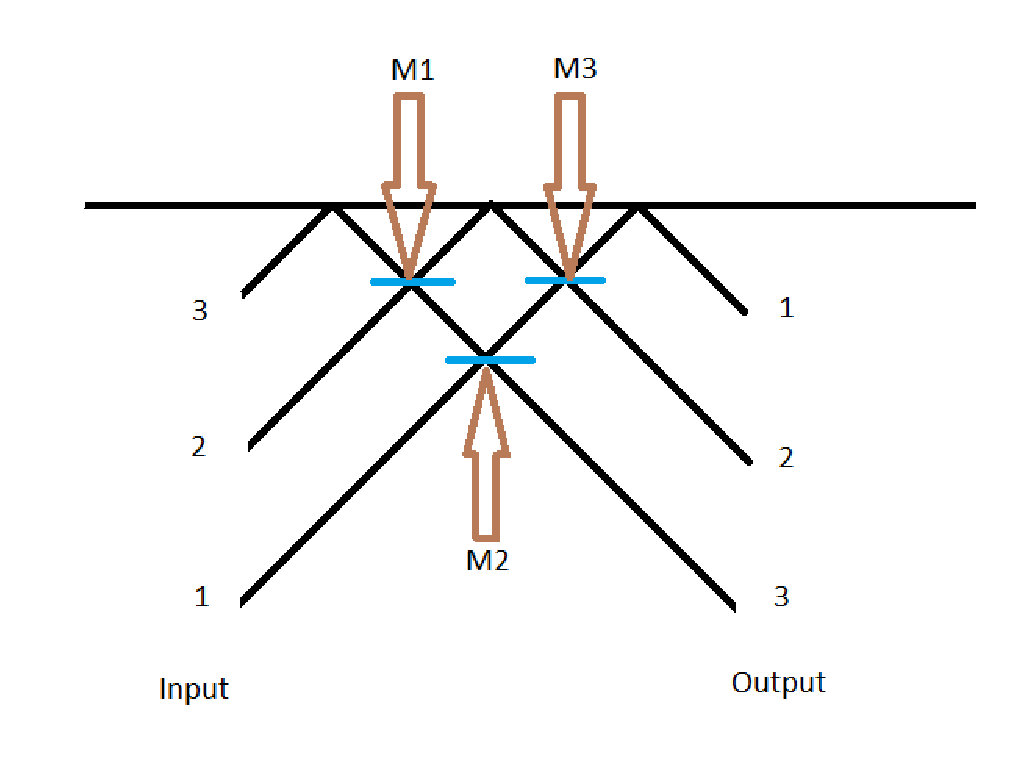
\includegraphics[width=8cm,height=6cm]{BeamSplitters}

where the coefficients of reflectivity and transmittance are given
by $\sqrt{R_{i}}=\sin\omega_{i}$ and $\sqrt{T_{i}}=\cos\omega_{i}$.

$U=M_{1}M_{2}M_{3}$=$\begin{pmatrix}\sqrt{p_{1}} & \frac{\sqrt{r_{2}}-\sqrt{p_{1}}cos\theta}{sin\theta} & \pm\frac{\sqrt{sin^{2}\theta-p_{1}-r_{2}+2\sqrt{p_{1}r_{2}}cos\theta}}{sin^{2}\theta}\\
\sqrt{r_{1}} & \frac{\sqrt{p_{2}}-\sqrt{r_{1}}cos\theta}{sin\theta} & \pm\frac{\sqrt{sin^{2}\theta-r_{1}-p_{2}+2\sqrt{p_{2}r_{1}}cos\theta}}{sin^{2}\theta}\\
\sqrt{q_{1}} & \frac{\sqrt{q_{2}}-\sqrt{q_{1}}cos\theta}{sin\theta} & \pm\frac{\sqrt{sin^{2}\theta-q_{1}-q_{2}+2\sqrt{q_{1}q_{2}}cos\theta}}{sin^{2}\theta}
\end{pmatrix}=$ 

$\begin{pmatrix}sin\omega_{1}sin\omega_{2} & cos\omega_{1}sin\omega_{3}+sin\omega_{1}cos\omega_{2}cos\omega_{3} & cos\omega_{1}cos\omega_{3}-sin\omega_{1}cos\omega_{2}sin\omega_{3}\\
cos\omega_{1}sin\omega_{2} & -sin\omega_{1}sin\omega_{3}+cos\omega_{1}cos\omega_{2}cos\omega_{3} & -sin\omega_{1}cos\omega_{3}-cos\omega_{1}cos\omega_{2}sin\omega_{3}\\
cos\omega_{2} & -sin\omega_{2}cos\omega_{3} & sin\omega_{2}sin\omega_{3}
\end{pmatrix}$ 

The coefficients of reflectivity and transmittance can be calculated
by matching the corresponding elements of the unitary and it's decomposition.
We can get all the elements by using just $U_{31},U_{32},U_{21}$ 

$U_{31}=\sqrt{q_{1}}=\cos\omega_{2},\sin\omega_{2}=\sqrt{1-\cos\omega_{2}^{2}}=\sqrt{1-q_{1}}$ 

$U_{32}=\frac{\sqrt{q_{2}}-\sqrt{q_{1}}cos\theta}{sin\theta}=-\sin\omega_{2}\cos\omega_{3}=-\sqrt{1-q_{1}}\cos\omega_{3}\Rightarrow$
$\cos\omega_{3}=-\frac{1}{\sqrt{1-q_{1}}}[\frac{\sqrt{q_{2}}-\sqrt{q_{1}}cos\theta}{sin\theta}]$

$\sin\omega_{3}=\sqrt{1-\cos\omega_{3}}=-\frac{\sqrt{sin^{2}\theta-q_{1}-q_{2}+2\sqrt{q_{1}q_{2}}cos\theta}}{\sqrt{1-q_{1}}sin\theta}$

$U_{21}=\sqrt{r_{1}}=\cos\omega_{1}\sin\omega_{2}=\cos\omega_{1}\sqrt{1-q_{1}}\Rightarrow$
$\cos\omega_{1}=\sqrt{\frac{r_{1}}{1-q_{1}}}$

$\sin\omega_{1}=\sqrt{1-\cos\omega_{1}}=\sqrt{\frac{p_{1}}{1-q_{1}}}$ 

Substituting the coefficients of reflectivity and transmittance the
beamsplitters are:

$M_{1}=\begin{pmatrix}\sqrt{\frac{p_{1}}{1-q_{1}}} & \sqrt{\frac{r_{1}}{1-q_{1}}} & 0\\
\sqrt{\frac{r_{1}}{1-q_{1}}} & -\sqrt{\frac{p_{1}}{1-q_{1}}} & 0\\
0 & 0 & 1
\end{pmatrix},M_{2}=\begin{pmatrix}\sqrt{1-q_{1}} & 0 & \sqrt{q_{1}}\\
0 & 1 & 0\\
\sqrt{q_{1}} & 0 & -\sqrt{1-q_{1}}
\end{pmatrix},M_{3}=\begin{pmatrix}1 & 0 & 0\\
0 & \frac{\sqrt{sin^{2}\theta-q_{1}-q_{2}+2\sqrt{q_{1}q_{2}}cos\theta}}{\sqrt{1-q_{1}}sin\theta} & -\frac{1}{\sqrt{1-q_{1}}}[\frac{\sqrt{q_{2}}-\sqrt{q_{1}}cos\theta}{sin\theta}]\\
0 & -\frac{1}{\sqrt{1-q_{1}}}[\frac{\sqrt{q_{2}}-\sqrt{q_{1}}cos\theta}{sin\theta}] & -\frac{\sqrt{sin^{2}\theta-q_{1}-q_{2}+2\sqrt{q_{1}q_{2}}cos\theta}}{\sqrt{1-q_{1}}sin\theta}
\end{pmatrix}$

All the coefficients can be expressed in terms of the $FRIO$. Using
the optimal relationship between the individual failure rates $\eta_{1}q_{1}=\eta_{2}q_{2}=Q/2$,$q_{1}=Q/2\eta_{1},q_{2}=Q/2\eta_{2}$
and the above expressions of success and error rates. 

$\cos\omega_{1}=\sqrt{\frac{r_{1}}{1-Q/2\eta_{1}}}$ , $\sin\omega_{1}=\sqrt{\frac{p_{1}}{1-Q/2\eta_{1}}}$

$\cos\omega_{2}=\sqrt{Q/2\eta_{1}}$, $\sin\omega_{2}=\sqrt{1-Q/2\eta_{1}}$

$\cos\omega_{3}=-\frac{\sqrt{Q/2\eta_{2}}-Q_{o}/2\eta_{1}\sqrt{Q/2\eta_{2}}}{\sqrt{(1-Q/2\eta_{1})(1-Q_{o}^{2}/4\eta_{1}\eta_{2})}}$,
$\sin\omega_{3}=\frac{\sqrt{1-Q_{o}^{2}/4\eta_{1}\eta_{2}-Q/(2\eta_{1}\eta_{2})+QQ_{o}/(2\eta_{1}\eta_{2})}}{\sqrt{(1-Q/2\eta_{1})(1-Q_{o}^{2}/4\eta_{1}\eta_{2})}}$

.

.

$M_{1}=\begin{pmatrix}\sqrt{\frac{p_{1}}{1-Q/2\eta_{1}}} & \sqrt{\frac{r_{1}}{1-Q/2\eta_{1}}} & 0\\
\sqrt{\frac{r_{1}}{1-Q/2\eta_{1}}} & -\sqrt{\frac{p_{1}}{1-Q/2\eta_{1}}} & 0\\
0 & 0 & 1
\end{pmatrix},$

$M_{2}=\begin{pmatrix}\sqrt{1-Q/2\eta_{1}} & 0 & \sqrt{Q/2\eta_{1}}\\
0 & 1 & 0\\
\sqrt{Q/2\eta_{1}} & 0 & -\sqrt{1-Q/2\eta_{1}}
\end{pmatrix},$

\[
M_{3}=\begin{pmatrix}1 & 0 & 0\\
0 & \frac{\sqrt{1-Q_{o}^{2}/4\eta_{1}\eta_{2}-Q/(2\eta_{1}\eta_{2})+QQ_{o}/(2\eta_{1}\eta_{2})}}{\sqrt{(1-Q/2\eta_{1})(1-Q_{o}^{2}/4\eta_{1}\eta_{2})}} & -\frac{\sqrt{Q/2\eta_{2}}-Q_{o}/2\eta_{1}\sqrt{Q/2\eta_{2}}}{\sqrt{(1-Q/2\eta_{1})(1-Q_{o}^{2}/4\eta_{1}\eta_{2})}}\\
0 & -\frac{\sqrt{Q/2\eta_{2}}-Q_{o}/2\eta_{1}\sqrt{Q/2\eta_{2}}}{\sqrt{(1-Q/2\eta_{1})(1-Q_{o}^{2}/4\eta_{1}\eta_{2})}} & -\frac{\sqrt{1-Q_{o}^{2}/4\eta_{1}\eta_{2}-Q/(2\eta_{1}\eta_{2})+QQ_{o}/(2\eta_{1}\eta_{2})}}{\sqrt{(1-Q/2\eta_{1})(1-Q_{o}^{2}/4\eta_{1}\eta_{2})}}
\end{pmatrix}.
\]
\vspace{0.05in}
 

Let us now check the bounds of the general unitary matrix for equal
priors to see if it reproduces the unitary in \ref{eq:U(equal prior)}.
Indeed, everything checks out and the equal priors unitary matrix
is reproduced: 
\begin{equation}
U=\begin{pmatrix}\sqrt{p} & \frac{\sqrt{r}-\sqrt{p}Q_{o}}{\sqrt{1-Q_{o}^{2}}} & \sqrt{\frac{Q}{1+Q_{o}}}\\
\sqrt{r} & \frac{[\sqrt{p}-\sqrt{r}Q_{o}]}{\sqrt{1-Q_{o}^{2}}} & \sqrt{\frac{Q}{1+Q_{o}}}\\
\sqrt{Q} & \sqrt{\frac{Q(1-Q_{o})}{1+Q_{o}}} & -\frac{\sqrt{p}+\sqrt{r}}{\sqrt{1+Q_{o}}}
\end{pmatrix},
\end{equation}





\subsection{Minimum Error}

Solution to the minimim error problem was derived in Chapter II. Here
we use the explicit solution to error and success rates to construct
the unitary operator which in turn will be expressed in terms of beamsplitters.
We start with the Neumart setup where a unitary operator entangles
the input states with the ancilla. Let the input states be $|\psi_{1}\rangle_{in}=|1\rangle$
and $|\psi_{2}\rangle_{in}=\cos\theta|1\rangle+\sin\theta|2\rangle$

\begin{align}
U|1\rangle_{in}|0\rangle & =\sqrt{p_{1}}|1\rangle+\sqrt{r_{1}}|2\rangle\\
U(\cos\theta|1\rangle+\sin\theta|2\rangle)|0\rangle & =\sqrt{r_{2}}|1\rangle+\sqrt{p_{2}}|2\rangle
\end{align}


Where the error and success rates were calculated in chapter two:

\begin{eqnarray}
r_{i} & = & \frac{1}{2}[1-\frac{1-2\eta_{j}s^{2}}{\sqrt{1-4\eta_{1}\eta_{2}s^{2}}}]\\
p_{i} & = & \frac{1}{2}[1-\frac{1-2\eta_{j}s^{2}}{\sqrt{1-4\eta_{1}\eta_{2}s^{2}}}]
\end{eqnarray}


To get the unitary elements multiply on the left by $\langle1|$ and
$\langle2|$ 

First column is:

$\langle1|U|1\rangle=U_{11}=\sqrt{p_{1}}$ 

$\langle2|U|1\rangle=U_{21}=\sqrt{r_{1}}$

Using the elements of the first column the second column can be calculated
and is:

$\cos\theta\langle1|U|1\rangle+\sin\theta\langle1|U|2\rangle=\cos\theta U_{11}+\sin\theta U_{12}=\cos\theta\sqrt{p_{1}}+\sin\theta U_{12}=\sqrt{r_{2}}\Rightarrow$
$U_{12}=\frac{\sqrt{r_{2}}-\cos\theta\sqrt{p_{1}}}{\sin\theta}$

$\cos\theta\langle2|U|1\rangle+\sin\theta\langle2|U|2\rangle=\cos\theta U_{21}+\sin\theta U_{22}=\cos\theta\sqrt{r_{1}}+\sin\theta U_{22}=\sqrt{p_{2}}\Rightarrow$
$U_{22}=\frac{\sqrt{p_{2}}-\cos\theta\sqrt{r_{1}}}{\sin\theta}$

The Unitary matrix is:

\begin{equation}
U=\begin{pmatrix}U_{11} & U_{12}\\
U_{21} & U_{22}
\end{pmatrix}=\begin{pmatrix}\sqrt{p_{1}} & \frac{\sqrt{r_{2}}-\cos\theta\sqrt{p_{1}}}{\sin\theta}\\
\sqrt{r_{1}} & \frac{\sqrt{p_{2}}-\sin\theta\sqrt{r_{1}}}{\sin\theta}
\end{pmatrix}
\end{equation}


Only one beam splitter is neccesary. 




\subsection{summary}

We derived the optimal rate of error for a fixed failure rate when
discriminating between two pure states with fixed a-priori probabilities.
Along the way we found expressions for the individual error rates.
Then we created an experimental implementation of this procedure using
the six-rail representation, and found that three beam-splitters are
sufficient to perform this experiment. 


\chapter*{Lagrange Multipliers}

In our works we have relied quite heavily in the Lagrange multipliers
when optimizing a function which was under the restriction of a constraint.
We now show why it works. The method can be applied to a function
of any number of variable but it can be more clearly explained in
two variables. Suppose that we need to find the stationary points
of a function $f(x,y),$ where $x$ and $y$ are the two variables,
subject to the constraint $g(x,y)=0.$ If the constraint is simple
then we can solve for $x$ in terms of $y,$ plug it into the function
then solve $\partial f/\partial y=0.$ However for slightly more complicated
constraint this can easily lead to a very high order equation with
cannot be solved analytically. In the case of exact cloning, doing
just so leads to a sixth order equation which is of little use. 

To find the stationary points of a function of two variable such as
$f(x,y),$ we could just take the total differentia $df$ and set
it to zero

\begin{equation}
df=\frac{\partial f}{\partial x}dx+\frac{\partial f}{\partial y}dy=0\label{eq:lagrange 1}
\end{equation}


which leads to two conditions:

\begin{equation}
\frac{\partial f}{\partial x}=0,\ \ \frac{\partial f}{\partial y}=0\label{eq:lagrange 0}
\end{equation}


However there is a constraint which means that the differentials $dx$
and $dy$ are not independent, they are related to the total differential
of $g$ by:

\begin{equation}
dg=\frac{\partial g}{\partial x}dx+\frac{\partial g}{\partial y}dy=0\label{eq:lagrange 2}
\end{equation}


Multiplying \ref{eq:lagrange 2} by the Lagrange parameter $\lambda$
and adding it to \ref{eq:lagrange 1} we get 

\begin{equation}
d(f+\lambda g)=(\frac{\partial f}{\partial x}+\lambda\frac{\partial g}{\partial x})dx+(\frac{\partial f}{\partial y}+\lambda\frac{\partial g}{\partial y})dy
\end{equation}


This equation can be satisfied by choosing the Lagrange multiplier
$\lambda$ such that the following two conditions are satisfied:

\begin{equation}
\frac{\partial f}{\partial x}+\lambda\frac{\partial g}{\partial x}=0\label{eq:lagrange x}
\end{equation}


and:

\begin{equation}
\frac{\partial f}{\partial y}+\lambda\frac{\partial g}{\partial y}=0\label{eq:lagrange y}
\end{equation}


To get the stationary points of $f(x,y)$ follow this procedure:
\begin{itemize}
\item Solve the two equations:\ref{eq:lagrange x} and \ref{eq:lagrange y}
in terms of $\lambda,$ $x(\lambda)$ and $y(\lambda)$ 
\item Plug $x(\lambda)$ and $y(\lambda)$ into the constraint $g(x,y)$ 
\item Solve for $\lambda$ 
\item Plug the value of $\lambda$ into $x(\lambda)$ and $y(\lambda)$ 
\item Plug $x(\lambda)$ and $y(\lambda)$ into the function which was to
be optimized $f(x,y)$
\end{itemize}
Now that we have seen how the Lagrange multipliers method works, we
can simplify the procedure by optimizing the function following function:

\begin{equation}
F(x,y)=f(x,y)+\lambda g(x,y)\label{eq:lagrange full}
\end{equation}


with respect to the the independent variable $x$ and $y.$ Differentiating
\ref{eq:lagrange full} with respect to $x$ and $y,$ we obtain equations
\ref{eq:lagrange x} and \ref{eq:lagrange y}. The rest of the procedure
is the same. This is the exact procedure we used for our works, for
example in optimizing the error rate $P_{E}(r_{1},r_{2})$ with one
constraint $s(r_{1},r_{2}).$ 

A more general procedure involving a function of $n$ variables, $f(x_{1},x_{2},...,x_{n}),$
and $j$ constrains goes in similar lines. We start by setting up
\ref{eq:lagrange full} 

\begin{equation}
F(x_{1},x_{2},...,x_{n})=f(x_{1},x_{2},...,x_{n})+\sum_{\lambda_{j}=1}^{m}\lambda_{j}g_{j}(x_{1},x_{2},...,x_{n}).
\end{equation}


Optimizing the function $f(x_{1},x_{2},...,x_{n})$ we differentiate
with respect to all the independent variables $(x_{1},x_{2},...,x_{n})$
and follow the procedure defined above. 


\chapter*{Reck-Zeilinger Algorithm }

In their letter \cite{Reck1994} prove that any discrete finite-dimensional
unitary operator can be constructed using optical devices only. Then
they provide a general algorithm which decomposes any $N$ $X$ $N$
unitary matrix into a product of two-dimensional $U(2)$ transformations
which can be expressed as beam splitters, phase shifters and mirrors.
This optical multi-port can act upon various fields such as electrons,
neutrons, atoms, photons etc. The authors decide to work with photons
purely for convenience and widespread availability of high power lasers.
It is this very proof which allows us to implement our various works
in state discrimination and cloning. In addition the proof has greatly
simplified the experimental realizations of many quantum computation,
quantum information and quantum cryptography schemes. Besides these
very practical applications it has also answered a long standing question:
Does an experiment measuring the variables corresponding to any arbitrary
Hermitian operator exists? They show that indeed an experimental realization
does exist for an arbitrary operator in a finite dimensional Hilbert
space. 

It has long been known that a lossless beam splitter and a phase shifter
can be implement any $U(2)$ transformation: a beam splitter and a
phase shifter at one output port transforms the input operators into
output operators as 

\begin{equation}
\begin{pmatrix}a'_{1}\\
a'_{2}
\end{pmatrix}=\begin{pmatrix}e^{i\phi}\sin\omega & e^{i\phi}\cos\omega\\
\cos\omega & -\sin\omega
\end{pmatrix}\begin{pmatrix}a_{1}\\
a_{2}
\end{pmatrix}
\end{equation}


where, $\phi$ is the phase shifter which can be realized as an external
phase shifter after the beam splitter, $\omega$ represents the transmittance
and reflectivity coefficient, $\sqrt{T}=\cos\omega,$ $\sqrt{R}=\sin\omega.$
In their Letter Reck, $et$ $al.$ considered the use of a Mach-Zehner
interferometer to simulate the effect of a beam splitter which splits
the incoming beam according to the given parameters of transmittance
and reflectivity. For an actual two by two beam splitter the coefficients
of transmittance and reflectivity should be $\sqrt{T}=\sin\omega$
and $\sqrt{R}=\sin\theta.$

The authors show that starting with an $N$ $\times$ $N$ unitary
matrix $U(N),$ it can be expressed into a succession of two-dimensional
matrices which correspond to beam splitters and phase shifters. Hence
the $U(N)$ unitary matrix can be realized in the full $N$ dimensional
Hilbert space through a succession of two-dimensional $U(2)$ matrices. 

The order in which the matrices are multiplied correspond to the sequence
in which the beamsplitters are set up. The task of realizing the experimental
setup of an arbitrary unitary matrix becomes that of factorizing the
matrix in terms of two dimensional beam splitter matrices with phase
shifters which can be realized after the beam splitters. 

Define an $N-$dimensional identity matrix $T_{pq}$ which multiplies
the $N$ dimensional unitary matrix from the right to reduce the dimensionality
to $N-1.$ In the identity matrix $T_{pq}$ the elements $I_{pq},\;I_{pp},\;I_{qp},\;I_{qq}$
are replaced by the corresponding beam splitter matrix elements $(\cos\omega,\sin\omega)$.
Thus:

\begin{equation}
U(N)\times T_{N,N-1}\times T_{N,N-2}\times...T_{N,1}=\begin{pmatrix}U(N-1) & 0\\
0 & e^{i\phi}
\end{pmatrix}
\end{equation}


This reduces the dimensionality of $U(N)$ to $U(N-1).$ The process
is repeated again until all the off diagonal elements of the original
unitary matrix are zero. 

\begin{equation}
U(N)\cdot T_{N,N-1}\cdot T_{N,N-2}\cdot...T_{N,1}\cdot T_{N-1,N-2}\cdot T_{N-2,N-2}\cdot...T_{2,1}\cdot...T_{2,1}=\begin{pmatrix}e^{i\alpha_{1}} & 0 & .. & 0\\
\vdots & e^{i\alpha_{2}}\\
 &  & \ddots\\
0 & \cdots &  & e^{i\alpha N}
\end{pmatrix}
\end{equation}


Let:

\begin{equation}
D=\begin{pmatrix}e^{-i\alpha_{1}} & 0 & .. & 0\\
\vdots & e^{-i\alpha_{2}}\\
 &  & \ddots\\
0 & \cdots &  & e^{-i\alpha N}
\end{pmatrix}
\end{equation}


we have 

\begin{equation}
U(N)\cdot T_{N,N-1}\cdot T_{N,N-2}\cdot...T_{N,1}\cdot T_{N-1,N-2}\cdot T_{N-2,N-2}\cdot...T_{2,1}\cdot D=I
\end{equation}


The unitary matrix can be expressed in terms of $Tp,q$ and $D:$ 

\begin{equation}
U(N)=D^{-1}\cdot T_{2,1}....\cdot T_{N-2,N-2}^{-1}\cdot T_{N-1,N-2}^{-1}\cdot T_{N,1}^{-1}....\cdot T_{N,N-2}^{-1}\cdot T_{N,N-1}^{-1}\label{eq:reck-seilinger algorithm}
\end{equation}
 Since the product of matrices represents the order of which the beam
splitters are set up, then \ref{eq:reck-seilinger algorithm} is all
one needs to implements a finite dimensional unitary matrix. Since
this algorithm is recursive, it can factorize any finite dimensional
unitary operator. For example a $3\times3$ unitary matrix, three
beam splitters are needed $T_{21},T_{31},T_{32},$ a $4\times4$ unitary
matrix requires six beamsplitters $T_{4,3},T_{4,2},T_{4,1},T_{32},T_{31},T_{21}$
in reversed order. In general the maximum number of beam splitters
required for any $N$ dimensional unitary operator is $\begin{pmatrix}N\\
2
\end{pmatrix}=\frac{N(N-1)}{2}.$ In practice this method involves a triangular array of beamsplitters,
with each diagonal row effectively reducing the dimension of the Hilbert
space by one.  

Let us now give an example to see explicitly how this algorithm works.
For a three dimensional unitary operator $U(3),$ the algorithm in
\ref{eq:reck-seilinger algorithm} gives:

\begin{equation}
U(3)=D^{-1}\times T_{2,1}^{-1}\times T_{3,1}^{-1}\times T_{3,2}^{-1}\label{eq:U(3)}
\end{equation}


where:

$D^{-1}=\begin{pmatrix}e^{i\alpha_{1}} & 0 & .. & 0\\
\vdots & e^{i\alpha_{2}}\\
 &  & \ddots\\
0 & \cdots &  & e^{i\alpha N}
\end{pmatrix},\ T_{21}=\begin{pmatrix}\sin\omega_{1} & \cos\omega_{1} & 0\\
\cos\omega_{1} & -\sin\omega_{1} & 0\\
0 & 0 & 1
\end{pmatrix},$

\bigskip{}


$T_{31}=\begin{pmatrix}\sin\omega_{2} & 0 & \cos\omega_{2}\\
0 & 1 & 0\\
\cos\omega_{2} & 0 & -\sin\omega_{2}
\end{pmatrix},\thinspace T_{32}=\begin{pmatrix}1 & 0 & 0\\
0 & \sin\omega_{3} & \cos\omega_{3}\\
0 & \cos\omega_{3} & -\sin\omega_{3}
\end{pmatrix}.$

Now plug this $2\times2$ matrices into \ref{eq:U(3)}.

\begin{equation}
\begin{pmatrix}U_{11} & U_{12} & U_{13}\\
U_{21} & U_{22} & U_{23}\\
U_{31} & U_{32} & U_{33}
\end{pmatrix}=\begin{pmatrix}e^{i\alpha_{1}} & 0 & .. & 0\\
\vdots & e^{i\alpha_{2}}\\
 &  & \ddots\\
0 & \cdots &  & e^{i\alpha N}
\end{pmatrix}\times\begin{pmatrix}sin\omega_{1}sin\omega_{2} & cos\omega_{1}sin\omega_{3}+sin\omega_{1}cos\omega_{2}cos\omega_{3} & cos\omega_{1}cos\omega_{3}-sin\omega_{1}cos\omega_{2}sin\omega_{3}\\
cos\omega_{1}sin\omega_{2} & -sin\omega_{1}sin\omega_{3}+cos\omega_{1}cos\omega_{2}cos\omega_{3} & -sin\omega_{1}cos\omega_{3}-cos\omega_{1}cos\omega_{2}sin\omega_{3}\\
cos\omega_{2} & -sin\omega_{2}cos\omega_{3} & sin\omega_{2}sin\omega_{3}
\end{pmatrix}
\end{equation}


To get the elements of the we match the corresponding entries $U_{ij}$
with the elements on right hand side. 



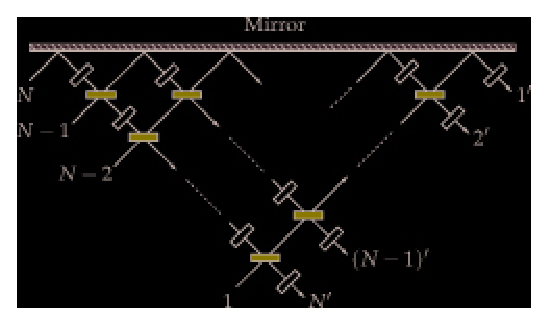
\includegraphics[width=8cm,height=6cm]{fig1-coherent}

\bibliographystyle{plain}
\bibliography{/Users/ashehu/Desktop/mendeley}

\end{document}
